\documentclass[12pt, a4paper]{article}
\usepackage[T1,T2A]{fontenc}
\usepackage[utf8]{inputenc}
\usepackage[english,russian]{babel}
\usepackage{amsmath}
\usepackage{amsfonts}
\usepackage{amsthm}
\usepackage{bnf}
\usepackage{amssymb}
\usepackage{makeidx}
\usepackage{tikz}
\usepackage{amsthm}
\usepackage{enumerate}
\usepackage{mathtext}
\usepackage{mathtools}
\usepackage{mathabx}
\usepackage[left=2cm,right=2cm,top=2cm,bottom=2cm,bindingoffset=0cm]{geometry}
\usepackage{proof}
\usepackage{paracol}
\usepackage{enumitem}
\usepackage{float}
\usepackage{colortbl}
\usepackage{minted}
\usepackage{tikz}
\usetikzlibrary{graphs}
\usetikzlibrary{graphs.standard}
\usetikzlibrary{automata,positioning}

\title{Введение в Теорию Типов\\\it{Конспект лекций}}
\author{Штукенберг Д.~Г.\\Университет ИТМО}
\DeclareMathOperator{\FV}{FV}

\begin{document}

\theoremstyle{definition}
\newtheorem{definition}{Определение}[section]
\newtheorem{note}{Замечание}[section]

\newtheorem{axiom}{Аксиома}[section]
\newtheorem{theorem}{Теорема}[section]
\newtheorem{lemma}[theorem]{Лемма}
\newtheorem{statement}{Утверждение}[section]
\newtheorem{oun_paragraph}{Пункт}[section]
\newtheorem{cons}{Следствие}[section]
\newtheorem*{example}{Пример}

\newcommand{\comb}[1]{\operatorname{\mathcal{#1}}}
\newcommand{\func}[1]{\operatorname{#1}}
\newcommand{\reduction}[1]{{\color{OrangeRed}#1}}
\newcommand{\set}[1]{\left\{#1\right\}}

\def\from#1{\par \parbox{0.7\textwidth}{\par \hfill\raggedleft \it #1}} 


\newenvironment{epigraph}% 
{\begin{list}{}{\setlength{\leftmargin}{0.3\textwidth}}\item[]}% 
{\end{list}} 

\maketitle
\section{Введение}

Эти лекции были рассказаны студентам групп М3334--М3337, M3339
в 2018 году в Университете ИТМО, на Кафедре компьютерных технологий Факультета информационных технологий и программирования.

Конспект подготовили студенты Кафедры: Егор Галкин (лекции 1 и 2),
Илья Кокорин (лекции 3 и 4), Никита Дугинец (лекции 5 и 6), Степан Прудников (лекции 7 и 8).

(возможно, история сложнее)

\section{Лекция 1}

\subsection{$\lambda$-исчисление}

\begin{definition}[$\lambda$-выражение]
	$\lambda$-выражение "--- выражение, удовлетворяющее грамматике:
	\begin{bnf}
	\begin{alignat*}{3}
		\Phi ::= & x
		       | & \left(\Phi\right) 
		       | & \lambda{}x.\Phi 
		       | & \Phi \ \Phi        
	\end{alignat*}
	\end{bnf}
\end{definition}

Иногда для упращения записи мы будем опускать скобки. В этом случае, перед разбором выражения, следует расставить все опущенные скобки. При их рассатвлении будем придерживаться правил:
\begin{enumerate}
	\item В аппликации расставляем скобки слева направо: $A \ B \ C \implies (A \ B) \ C$.
	\item Абстракции жадные "--- поглащают скобками все что могут до конца строки: 
	$\lambda{}a.\lambda{}b.a \ b \implies \lambda{}a.(\lambda{}b.(a \ b))$.
	\vspace{1mm}
	\begin{example}
		$\lambda{}x.(\lambda{}f.((f x) (f x) \lambda{}y.(y f)))$
	\end{example}
\end{enumerate}

Договоримся, что:
\begin{itemize}
	\item Переменные "--- $x$, $a$, $b$, $c$.
	\item Термы (части $\lambda$-выражения) "--- $X$, $A$, $B$, $C$.
	\item Фиксированные переменные обозначаются буквами из начала алфавита, метапеременные "--- из конца.
\end{itemize}

Есть понятия связанного и свободного вхождения переменной (аналогично исчислению предикатов).

\begin{definition}
	Если вхождение $x$ находится в области действия абстракции по $x$, то такое вхождение называется связанным, иначе вхождение называется свободным.
\end{definition}

\begin{definition}
	Терм $Q$ называется свободным для подстановски в $\Phi$ вместо $x$, если после подстановки $Q$ ни одно вхождение не станет связанным.
\end{definition}

\begin{example}
	$\lambda{}x.A$ связывает все свободные вхождения $x$ в $A$.
\end{example}

\begin{definition}
	Функция $V(A)$ "--- множество переменных, входящих в $A$.
\end{definition}

\begin{definition} 
	Функция $\FV(A)$ "--- множество свободных переменных, входящих в $A$:
	\[
	\FV(A) =
	\begin{cases}
	\set{x}                  & \text{если } A \equiv x \\
	\FV(P) \cup \FV(Q)       & \text{если } A \equiv PQ \\
	\FV(P) \setminus \set{x} & \text{если } A \equiv \lambda x . P
	\end{cases}
	\]
\end{definition}

$\lambda$-выражение можно понимать как функцию.
Абстракция "--- это функция с аргументом, аппликация "--- это передача аргумента.

\begin{definition}[$\alpha$-эквивалентность]
	$A=_{\alpha}B$, если имеет место одно из следующих условий:
	\begin{enumerate}
		\item $A\equiv{}x$, $B\equiv{}y$ и $x\equiv{}y$.
		\item $A\equiv{}P_{1}Q_{1}$, $B\equiv{}P_{2}Q_{2}$ и $P_{1}=_{\alpha}P_{2}$, $Q_{1}=_{\alpha}Q_{2}$.
		\item $A\equiv \lambda{}x.P_{1}$, $B\equiv \lambda{}y.P_{2}$ и $P_{1} [x\coloneqq{}t] =_{\alpha}P_2 [y\coloneqq{}t]$, где $t$ "--- новая переменная.
	\end{enumerate} 
\end{definition}

\begin{example}
	$\lambda{}x.\lambda{}y.xy=_{\alpha}\lambda{}y.\lambda{}x.yx$.
	\begin{proof} 
		\
		\begin{enumerate}
			\item $t z =_ \alpha t z$ верно по второму условию.
			\item Тогда получаем, что $\lambda{}y.t y =_\alpha \lambda{}x. t x$ по третьему условию, так как из предыдущего пункта следует $t y[y \coloneqq z] =_\alpha tx[x \coloneqq z]$.
			\item Из второго пункта пункта получаем что $\lambda{}x.\lambda{}y.xy=_{\alpha}\lambda{}y.\lambda{}x.yx$ по третьему условию, так как $\lambda{}y.xy[x \coloneqq t] =_\alpha \lambda{}x.yx[y \coloneqq t]$.
		\end{enumerate}
	\end{proof}
\end{example}

\begin{definition}[$\beta$-редекс]
	$\beta$-редекс "--- выражение вида: $\left(\lambda{}x.A\right)B$
\end{definition}

\begin{definition}[$\beta$-редукция]
	$A\to_{\beta}B$, если имеет место одно из следующих условий:
	\begin{enumerate}
		\item $A\equiv{}P_{1}Q_{1}$, $B\equiv{}P_{2}Q_{2}$ и либо $P_{1}=_{\alpha}P_{2}$, $Q_{1}\to_{\beta}Q_{2}$, либо
		$P_{1}\to_{\beta}P_{2}$, $Q_{1}=_{\alpha}Q_{2}$
		\item $A\equiv\left(\lambda{}x.P\right) Q$, $B\equiv P[x\coloneqq{}Q]$ причем $Q$ свободна для подстановки вместо $x$ в $P$ 
		\item $A\equiv\lambda{}x.P$, $B\equiv\lambda{}x.Q$ и $P\to_{\beta}Q$
	\end{enumerate}
	\begin{example} 
		$\left(\lambda{}x.x\right) y\to_{\beta} y$
	\end{example}
	\begin{example}
		 $a \left(\lambda{}x.x\right) y\to_{\beta} a y$
	\end{example}
\end{definition}

\subsection{Представление некоторых функций в лямбда исчислении}
Логические значения легко представить в терминах $\lambda$-исчисления. В самом деле, положим:
\begin{itemize}
	\item $\func{True}  \equiv \lambda{}a\lambda{}b.a$ 
	\item $\func{False} \equiv \lambda{}a\lambda{}b.b$
\end{itemize}

\newcommand{\If}{\lambda{}c.\lambda{}t.\lambda{}e.(c t) e}
\newcommand{\T}{\lambda{}a\lambda{}b.a}
\newcommand{\F}{\lambda{}a\lambda{}b.b}
\newcommand{\Fl}{\func{F}}
\newcommand{\Tl}{\func{T}}


Также мы можем выражать и более сложные функции \\


\begin{definition}
	$\func{If} \equiv \If$
\end{definition}

\begin{example}
	$\func{If} \ \Tl \ a \ b \to_{\beta} \ a$
	\begin{proof}
		\begin{alignat*}{2}
		 ((\If) \ \T)\ a \ b \to_{\beta} (\lambda{}t.\lambda{}e.(\T) \ t \ e) \ a \ b \to_{\beta} \ \\ (\lambda{}t.\lambda{}e.(\lambda{}b.t) \ e) \ a \ b \to_{\beta} \ (\lambda{}t.\lambda{}e.t) \ a \ b \to_{\beta} \ (\lambda{}e.a) \ b \to_{\beta} \ a
		\end{alignat*}
	\end{proof}
\end{example}

Как мы видим If $\Tl$ действительно возвращает результат первой ветки.


Другие логические операции:
\[
	\func{Not} = \lambda{}a.a \ \Fl \ \Tl \qquad
	\func{Add} = \lambda{}a.\lambda{}b.a \ b \ \Fl \qquad
	\func{Or}  = \lambda{}a.\lambda{}b.a \ \Tl \ b \qquad
\]



\subsection{Черчевские нумералы}

\begin{definition}[черчевский нумерал]
	\[
		\overline{n} = \lambda{}f.\lambda{}x.f^{n} x \text{, \quad где\quad}
		f^{n} x = 
		\begin{cases}
			f\left(f^{n-1} x\right) & \text{при } n > 0 \\
			x 						& \text{при } n = 0
		\end{cases}
	\]
\end{definition}

\begin{example}
	\[
	\overline{3} = \lambda f . \lambda x . f \left(f \left(f x\right)\right)
	\]
\end{example}

Несложно определить прибавление единицы к такому нумералу:
\[
	(+1) = \lambda{}n.\lambda{}f.\lambda{}x.f(nfx) \\
\]



Арифметические операции:
\begin{enumerate}
	\item $\func{IsZero} = \lambda{}n.n\mathinner{(\lambda{}x.\Fl)} \Tl$ 
	\item $\func{Add} =\lambda{}a.\lambda{}b.\lambda{}f.\lambda{}x.a \mathinner{f} (b \mathinner{f} x)$ 
	\item $\func{Pow} = \lambda{}a.\lambda{}b.b \mathinner{(\func{Mul}  \  a)} \mathinner{\overline{1}}$
	\item $\func{IsEven} = \lambda{}n.n \ \func{Not} \ \Tl$
	\item $\func{Mul} = \lambda{}a.\lambda{}b.a \mathinner{(\func{Add}\ b)} \mathinner{\overline{0}}$
\end{enumerate}

Для того, чтобы определить $(-1)$, сначала определим пару:
\[
\left<a,b\right> = \lambda f.f \mathinner{a} b \qquad
\func{First} = \lambda p . p \Tl \qquad
\func{Second} = \lambda p . p \Fl
\]%

Затем $n$ раз применим функцию $f\left(\left<a,b\right>\right) = \left<b,b+1\right>$ и возьмём первый элемент пары:
\[
(-1) = \lambda n . \func{First}
(n \mathinner{(\lambda p . \left<\left(\func{Second} p\right), \mathinner{(+1)} (\func{Second} p)\right>)}
\langle\overline{0},\overline{0}\rangle)
\]

\section{Лекция 2}

\subsection{Формализация $\lambda$-термов, классы $\alpha$-эквивалентности термов}

\begin{definition}[$\lambda$-терм]
	Рассмотрим классы эквивалентности $[A]_{=_{\alpha}}$ \\
	Будем говорить, что $[A]\to_{\beta}[B]$, если  существуют $A^{'}\in [A]$ и $B^{'} \in [B]$, что $A^{'}\to_{\beta}B^{'}$.
\end{definition}

\begin{lemma}
	$(=_{\alpha})$ "--- отношение эквивалентности.
\end{lemma}

Пусть в A есть $\beta$-редекc $(\lambda{}x.P)Q$, но $Q$ не свободен для подстановки вместо $x$ в $P$,
тогда найдем $y\notin V[P]$, $y\notin V[Q]$. Сделаем замену $P[x\coloneqq{}y]$.
Тогда замена $P[x\coloneqq{}y][y\coloneqq{}Q]$ допустима. То есть, можно сказать, что мы просто переименовали переменную $x$ в $P$ и получили свободу для подстановки, тем самым получив возможность редукции.

\begin{lemma}
	$P[x\coloneqq{}Q]=_{\alpha}P[x\coloneqq{}y][y\coloneqq{}Q]$, если замена допустима.
\end{lemma}

\subsection{Нормальная форма, $\lambda$-выражения без нормальной формы, \\комбинаторы $K$, $I$, $\Omega$}

\begin{definition}
	$\lambda$-выражение $A$ находится в нормальной форме, если оно не содержит $\beta$-редексов.
\end{definition}

\begin{definition}
	$A$ "--- нормальная форма $B$, если существует последовательность термов $A_{1}...A_{n}$ такая, что $B=_{\alpha}A_{1}\to_{\beta}A_{2}\to_{\beta}...\to_{\beta}A_{n}=_{\alpha}A$.
\end{definition}

\begin{definition}
	Комбинатор "--- $\lambda$-выражение без свободных переменных.
\end{definition}

\begin{definition} 
	\hfill
	\begin{itemize}
		\item $I \equiv \lambda{}x.x$ (Identitant)
		\item $K \equiv \lambda{}a.\lambda{}b.a$ (Konstanz)
		\item $\Omega \equiv (\lambda{}x.xx)(\lambda{}x.xx)$
	\end{itemize}
\end{definition}

\begin{lemma}
	$\Omega$ "--- не имеет нормальной формы.
\end{lemma}

\begin{proof}
	$\Omega$ Имеет единственный $\beta$-редекс, где $A \equiv xx$, $B \equiv (\lambda{}x.xx)$. Тогда единственный возможный путь редукции "--- подставить $B$ вместо $x$ в $A$. Но тогда мы получим $\Omega$. Следовательно, у $\Omega$ нет нормальной формы, так как в полученном выражении у нас всегда будет $\beta$-редекс.
\end{proof}

\subsection{$\beta$-редуцируемость}

\begin{definition}
	Будем говорить, что $A\twoheadrightarrow_{\beta}B$, если $\exists$ такие $X_{1}$\ldots $X_{n}$, что $A=_{\alpha}X_{1}\to_{\beta}X_{2}\to_{\beta}\ldots\to_{\beta}X_{n-1}\to_{\beta}X_{n}=_{\alpha}B$.
\end{definition}

$(\twoheadrightarrow_{\beta})$ "--- рефлексивное и транзитивное замыкание $(\to_{\beta})$. $(\twoheadrightarrow_{\beta})$ не обязательно приводит к нормальной форме
\begin{example}
	$\Omega\twoheadrightarrow_{\beta}\Omega$
\end{example}

\subsection{Ромбовидное свойство}

\begin{definition}[Ромбовидное свойство]
	Отношение $R$ обладает ромбовидным свойством, если $\forall a,b,c$, таких, что $aRb$, $aRc$, $b\neq{}c$, $\exists{}d$, что $bRd$ и $cRd$.
\end{definition}

\begin{example}
	$(\leq)$ на множестве натуральных чисел обладает ромбовидным свойством,
	$(>)$ на множестве натуральных чисел не обладает ромбовидным свойством.
\end{example}

\subsection{Теорема Чёрча-Россера, следствие о единственности \\нормальной формы}

\begin{theorem}[Черча-Россера]
	$(\twoheadrightarrow_{\beta})$ обладает ромбовидным свойством.
\end{theorem}


\begin{cons}
	Если у $A$ есть нормальная форма, то она единственная с точностью до $(=_{\alpha})$ (переименования переменных).
\end{cons}

\begin{proof}
	Пусть $A\twoheadrightarrow_{\beta}B$ и $A\twoheadrightarrow_{\beta}C$. $B$, $C$ "--- нормальные формы и $B\neq_{\alpha}C$. 
	Тогда по теореме Черча-Россера $\exists{}D$: $B\twoheadrightarrow_{\beta}D$ и $C\twoheadrightarrow_{\beta}D$. Тогда $B=_{\alpha}D$ и $C=_{\alpha} D$ $\Rightarrow$ $B=_{\alpha}C$. Противоречие.
\end{proof}

\begin{lemma}
	Если $B$ "--- нормальная форма, то не существует $Q$ такой, что $B\to_{\beta}Q$. Значит если $B\twoheadrightarrow_{\beta}Q$, то количество шагов редукции равно 0.
\end{lemma}

\begin{lemma}
	 \label{refl}
	Если $R$ "--- обладает ромбовидным свойством, то и $R^{*}$ (транзитивное, рефлексивное замыкание $R$) им обладает.
\end{lemma}

\begin{proof}
    Пусть $M_1 R^{*} M_n$ и $M_1 R N_1$. Тогда существуют такие $M_2 \ldots M_{n-1}$, что $M_1 R M_2$ \ldots $M_{n-1} R M_n$.
	Так как $R$ обладает ромбовидным свойством, $M_1 R M_2$ и $M_1 R N_1$, то существует такое $N_2$,
	что $N_1 R N_2$ и $M_2 R N_2$. Аналогично, существуют такие $N_3 \ldots N_n$, что $N_{i-1} R N_{i}$ и $M_i R N_i$.
	Мы получили такое $N_n$, что $N_1 R^{*} N_n$ и $M_n R^{*} N_n$.
	
	Пусть теперь $M_{1,1}R^{*}M_{1,n}$ и $M_{1,1}R^{*}M_{m,1}$, то есть имеются $M_{1,2}$\ldots$M_{1,n-1}$ и $M_{2,1}$\ldots$M_{m-1,1}$,
	что $M_{1,i-1} R M_{1,i}$ и $M_{i-1, 1} R M_{i, 1}$.
	Тогда существует такое $M_{2,n}$, что $M_{2,1} R^{*} M_{2,n}$ и $M_{1,n} R^{*} M_{2,n}$.
	Аналогично, существуют такие $M_{3,n}\ldots M_{m,n}$, что $M_{i,1} R^{*} M_{i,n}$ и $M_{1,n} R^{*} M_{i,n}$.
	Тогда $M_{1,n} R^{*} M_{m,n}$ и $M_{m,1} R^{*} M_{m,n}$.
\end{proof}

\begin{lemma}[Грустная лемма]
	$(\to_{\beta})$ не обладает ромбовидным свойством.
\end{lemma}

\begin{proof}
	Пусть $A=(\lambda{}x.x x)(\comb I \comb I)$. Покажем, что в таком случае не будет выполняться ромбовидное свойство:
	\
	\begin{figure}[ht]
		\centering
		\begin{tikzpicture}[->, every edge/.style={draw=black,thick}]
		\node[label={\scriptsize\tikz\node[circle,draw]{$A$};}]     at (0,   0) (A)  {$(\lambda x . x x)(\comb I \comb I)$};
		\node[label={135:\scriptsize\tikz\node[circle,draw]{$B$};}] at (-2, -1) (B)  {$(\comb I \comb I)(\comb I \comb I)$};
		\node[label={45:\scriptsize\tikz\node[circle,draw]{$C$};}]  at (2,  -1) (C)  {$(\lambda x . x x)  \comb I$};
		\node[label={180:\scriptsize\tikz\node[circle,draw]{$B1$};}]                                                       at (-3, -2) (B1) {$(\comb I \comb I)\comb I$};
		\node[label={0:\scriptsize\tikz\node[circle,draw]{$B2$};}]                                                       at (-1, -2) (B2) {$\comb I(\comb I \comb I)$};
		\node[label={0:\scriptsize\tikz\node[circle,draw]{$D$};}]                                                       at (0,  -3) (D)  {$\comb I \comb I$};
		\path (A)  edge (B)
		edge (C)
		(B)  edge (B1)
		edge (B2)
		(B1) edge (D)
		(B2) edge (D)
		(C)  edge (D);
		\end{tikzpicture}
		\caption{Нет такого $D$, что $B \to_{\beta} D$ и $C \to_{\beta} D$.}
	\end{figure}	
	\\
\end{proof}


\newcommand{\bpar}{\rightrightarrows_{\beta}}

\begin{definition}[Параллельная $\beta$-редукция]
	$A\bpar B$, если
	\begin{enumerate}
		\item $A=_{\alpha}B$
		\item $A\equiv{}P_{1}Q_{1}$, $B\equiv{}P_{2}Q_{2}$ и $P_{1}\bpar P_{2}$, $Q_{1}\bpar Q_{2}$
		\item $A\equiv{}\lambda{}x.P_{1}$, $B\equiv{}\lambda{}x.P_{2}$ и 
		$P_{1}\bpar P_{2}$
		\item $A=_{\alpha}(\lambda{}x.P_1)Q_1$, $B=_{\alpha}P_2[x\coloneqq{}Q_2]$ причем $Q_2$ свободна для подстановки вместо $x$ в $P_2$ и $P_1 \bpar P_2$, $Q_1 \bpar Q_2$
	\end{enumerate}
\end{definition}

\begin{lemma}
	\label{bparhelp}
	Если $P_{1}\bpar P_{2}$ и $Q_{1}\bpar Q_{2}$, то $P_{1}[x\coloneqq{}Q_{1}]\bpar P_{2}[x\coloneqq{}Q_{2}]$
\end{lemma}

\begin{proof}
	Будем доказывать индукцией по определению $\bpar $. Рассмотрим случаи:
	\begin{itemize}
		\item Пусть $P_{1}=_{\alpha}P_{2}$. Тогда лемма легко доказывается индукцией по структуре выражения.
		\item Пусть $P_{1}\equiv{}A_{1}B_{1}$, $P_{2}\equiv{}A_{2}B_{2}$. По определению $(\bpar)$ $A_{1} \bpar A_{2}$ и $B_{1} \bpar B_{2}$.
		Рассмотрим два случая:
		\begin{enumerate}
			\item $x \in \FV(A_{1})$. По индукционному предположению $A_{1}[x\coloneqq{}Q_{1}] \bpar A_{2}[x\coloneqq{}Q_{2}]$. Тогда $A_{1}[x\coloneqq{}Q_{1}]B_{1} \bpar A_{2}[x\coloneqq{}Q_{2}]B_{2}$. Тогда $A_{1}B_{1}[x\coloneqq{}Q_{1}] \bpar A_{2}B_{2}[x\coloneqq{}Q_{2}]$.
			\item $x \in \FV(B_{1})$. По индукционному предположению $B_{1}[x\coloneqq{}Q_{1}] \bpar B_{2}[x\coloneqq{}Q_{2}]$. Тогда $A_{1}B_{1}[x\coloneqq{}Q_{1}] \bpar A_{2}B_{2}[x\coloneqq{}Q_{2}]$.
		\end{enumerate}
		\item Пусть $P_{1}\equiv{}\lambda{}y.A_{1}$, $P_{2}\equiv{}\lambda{}y.A_{2}$. По определению $(\bpar)$ $A_{1}\bpar A_{2}$. Тогда по индукционному предположению $A_{1}[x\coloneqq{}Q_{1}] \bpar A_{2}[x\coloneqq{}Q_{2}]$. Тогда 
		$\lambda{}y.(A_{1}[x\coloneqq{}Q_{1}]) \bpar \lambda{}y.(A_{2}[x\coloneqq{}Q_{2}])$ по определению $(\bpar)$. Следовательно 	$\lambda{}y.A_{1}[x\coloneqq{}Q_{1}] \bpar \lambda{}y.A_{2}[x\coloneqq{}Q_{2}]$ по определению подстановки.
		\item Пусть $P_{1}=_\alpha(\lambda{}y.A_1)B_1$, $P_{2}=_\alpha A_2[y\coloneqq{}B_2]$ и $ A_1 \bpar A_2 $, $ B_1 \bpar B_2 $. По индукционному предположению получаем, что $A_1[x \coloneqq Q_1] \bpar A_2[x \coloneqq Q_2]$, $B_1[x \coloneqq Q_1] \bpar B_2[x \coloneqq Q_2]$. Следовательно, по определению $(\bpar)$ получаем, что $ (\lambda{}y.A_1[x\coloneqq Q_1])B_1[x \coloneqq Q_1] \bpar  A_2[y \coloneqq B_2][x \coloneqq Q_2]$
	\end{itemize}
\end{proof}

\begin{lemma}
	$(\bpar)$ обладает ромбовидным свойством.
\end{lemma}

\begin{proof}
	Будем доказывать индукцией по определению $(\bpar)$. Покажем, что если $M \bpar M_1$ и $M \bpar M_2$, то существует ${}M_3$, что $M_1 \bpar M_3$ и $M_2 \bpar M_3$. Рассмотрим случаи:
	\begin{itemize}
		\item Если $M\equiv M_1$, то просто возьмем $M_3\equiv M_2$.
		\item Если $M\equiv \lambda{}x.P, M_1 \equiv \lambda{}x.P_1, M_2 \equiv \lambda{}x.P_2$ и $P \bpar P_1, P \bpar P_2$, то по предположению индукции 
		существует $P_3$, что $P_1 \bpar P_3, P_2 \bpar P_3$, тогда возьмем $M_3\equiv \lambda{}x.P_3$.
		\item Если $M \equiv P Q, M_1 \equiv P_1 Q_1$ и по определению $(\bpar)$ $P \bpar P_1, Q \bpar Q_1$, то рассмотрим два случая:
		\begin{enumerate}
			\item $M_2 \equiv P_2 Q_2$. Тогда по предположению индукции существует $P_3$, что $P_1 \bpar P_3, P_2 \bpar P_3$. Аналогично для $Q$. Тогда возьмем $M_3 \equiv P_3 Q_3$.
			\item $P\equiv \lambda {}x.P'$ значит $P_1 \equiv \lambda{}x.P_1'$ и $ P' \bpar P_1'$. Пусть тогда $ M_2 \equiv P_2[x\coloneqq{} Q_2]$, по определению $(\bpar)$ $P' \bpar P_2, Q \bpar Q_2$. Тогда по предположению индукции и лемме $\ref{bparhelp}$ существует $M_3 \equiv P_3[x \coloneqq Q_3]$ такой, что $ P_1' \bpar P_3 $, $ Q_1 \bpar Q_3 $ и $ P_2 \bpar P_3 $, $ Q_2 \bpar Q_3 $.
		\end{enumerate}
	\item Если $ M \equiv (\lambda{}x.P)Q $, $ M_1 \equiv P_1[x\coloneqq Q_1] $ и $ P \bpar P_1 $, $ Q \bpar Q_1$, то рассмотрим случаи:
	\begin{enumerate}
		\item $ M_2 \equiv (\lambda{}x.P_2)Q_2 $, $P \bpar P_2$, $Q \bpar Q_2$. Тогда по предположению индукции и лемме $ \ref{bparhelp} $ существует такой $ M_3 \equiv P_3[x \coloneqq Q_3] $, что $ P_1 \bpar P_3 $, $ Q_1 \bpar Q_3 $ и $ P_2 \bpar P_3 $, $ Q_2 \bpar Q_3 $.
		\item $ M_2 \equiv P_2[x \coloneqq Q_2]$, $ P \bpar P_2 $, $ Q \bpar Q_2 $. Тогда по предположению индукции и лемме $ \ref{bparhelp} $ существует такой $ M_3 \equiv P_3[x \coloneqq Q_3] $, что $ P_1 \bpar P_3 $, $ Q_1 \bpar Q_3 $ и $ P_2 \bpar P_3 $, $ Q_2 \bpar Q_3 $.
	\end{enumerate}
	\end{itemize}
\end{proof}

\begin{lemma}
	\
	\begin{enumerate}
		\item $(\bpar )^{*} \subseteq (\to_{\beta})^{*}$
		\item $(\to_{\beta})^{*} \subseteq (\bpar )^{*}$
	\end{enumerate}
\end{lemma}

\begin{cons}
	$(\to_{\beta})^{*}=(\bpar )^{*}$
\end{cons}

Из приведенных выше лемм и следствия докажем теорему Черча-Россера.

\begin{proof}
	$(\to_{\beta})^{*} = (\twoheadrightarrow_{\beta})$. Тогда $(\twoheadrightarrow_{\beta})=(\bpar )^{*}$. Значит из того, что $(\bpar )$ обладает ромбовидным свойством и леммы $\ref{refl}$ следует, что $(\twoheadrightarrow_{\beta})$ обладает ромбовидным свойством.
\end{proof}

\subsection{Нормальный и аппликативный порядок вычислений}

\begin{example}
	Выражение $KI\Omega$ можно редуцировать двумя способами:
	\begin{enumerate}
		\item $\comb K \comb I \Omega =_{\alpha} ((\lambda{}a.\lambda{}b.a) \comb I) \Omega \to_{\beta} (\lambda{}b.\comb I)\Omega  \to_{\beta} \comb I$
		\item  $\comb K \comb I \Omega =_{\alpha} ((\lambda{}a.\lambda{}b.a) \comb I)((\lambda{}x.x \ x) (\lambda{}x.x \ x)) \twoheadrightarrow_{\beta} ((\lambda{}a.\lambda{}b.a) \comb I)((\lambda{}x.x \ x) (\lambda{}x.x \ x)) \to_{\beta} \comb K \comb I \Omega $
	\end{enumerate}
	
\end{example}

Как мы видим, в первом случае мы достигли нормальной формы, в то время как во втором мы получили бесконечную редукцию. Разница двух этих способов в порядке редукции. Первый называется нормальный порядок, а второй аппликативный. 

\begin{definition}[нормальный порядок редукции]
	Редукция самого левого $\beta$-редекса.
\end{definition}

\begin{definition}[аппликативный порядок редукции]
	Редукция самого левого $\beta$-редекса из самых вложенных.
\end{definition}

\begin{theorem}[Приводится без доказательства]
	Если нормальная форма существует, она может быть достигнута нормальным порядком редукции.
\end{theorem}

Нормальный порядок хоть и приводит к нормальной форме, если она существует, но бывают ситуации в которых аппликативный порядок вычисляется быстрее чем нормальный.

\begin{example}
	Рассмотрим $\lambda$-выражение $(\lambda{}x.x \ x \ x \ x) (\comb I \comb I)$. Попробуем редуцировать его нормальным порядком:
	 \[(\lambda{}x.x \ x \ x \ x) (\comb I \comb I) \to_{\beta} (\comb I \comb I)(\comb I \comb I)(\comb I \comb I)(\comb I \comb I) \to_{\beta} \comb I(\comb I \comb I)(\comb I \comb I)(\comb I \comb I) \to_{\beta} (\comb I \comb I)(\comb I \comb I)(\comb I \comb I) \to_{\beta} \ldots \to_{\beta} \comb I\] 
	Как мы увидим, в данной ситуации аппликативный порядок редукции оказывается значительно эффективней: 
	\[ (\lambda{}x.x \ x \ x \ x) (\comb I \comb I) \to_{\beta} (\lambda{}x.x \ x \ x \ x) \comb I \to_{\beta} \comb I \comb I \comb I \comb I\to_{\beta} \comb I \comb I \comb I \to_{\beta} \comb I \comb I \to_{\beta} \comb I \]
\end{example}

\section{Лекция 3}

\subsection{Y-комбинатор}

\begin{definition}
	Комбинатором называется $\lambda$-выражение, не имеющее свободных переменных
\end{definition}

\begin{definition}($Y$-комбинатор)
	\[
	Y = \lambda f . (\lambda x . f (x x)) (\lambda x . f (x x))
	\]
\end{definition}

Очевидно, $Y$-комбинатор является комбинатором.

\begin{theorem}
	$Y f =_{\beta} f (Y f)$
	
	\begin{proof}
		$\beta$-редуцируем выражение $Y f$
		\begin{align*}
			 =_{\beta} \textcolor{magenta}{(\lambda f . (\lambda x . f (x x)) (\lambda x . f (x x)))}\textcolor{blue}{f} \\ =_{\beta} \textcolor{magenta}{(\lambda x . f (x x))} \textcolor{blue}{(\lambda x . f (x x))} \\ =_{\beta} f ((\lambda x . f (x x))(\lambda x . f (x x))) \\ =_{\beta} f(Y f)
		\end{align*}
		Так как при второй редукции мы получили, что $Y f =_{\beta} (\lambda x . f (x x))(\lambda x . f (x x))$
	\end{proof}	
\end{theorem}

Следствием этого утверждения является теорема о неподвижной точкe для бестипового $\lambda$-исчисления

\begin{theorem}
	В $\lambda$-исчислении каждый терм $f$ имеет неподвижную точку, то есть такое $p$, что $f \; p =_{\beta} p$
	
	\begin{proof}
		Возьмём в качестве $p$ терм $Y f$. По предыдущей теореме, $f(Y f) =_{\beta} Y f$, то есть $Y f$ является неподвижной точкой для $f$. Для любого терма $f$ существует терм $Y f$, значит, у любого терма есть неподвижная точка.
	\end{proof}
\end{theorem}

\subsection{Рекурсия}

С помощью $Y$-комбинатора можо определять рекурсивные функции, например, функцию, вычисляющую факториал Чёрчевского нумерала. Для этого определим вспомогательную функцию

$fact' \equiv \lambda f. \lambda n. isZero\; n \; \overline{1} (mul \; n \; f((-1) n))$

Тогда $fact \equiv Y fact'$

Заметим, что $fact \; \overline{n} =_{\beta} fact' \; (Y \; fact') \; \overline{n} =_{\beta}fact' \; fact \; \overline{n} $, то есть в тело функции $fact'$ вместо функции $f$ будет подставлена $fact$ (заметим, что это значит, что именно функция $fact$ будет применена к $\overline{n - 1}$, то есть это соответствует нашим представлениям о рекурсии).

Для понимания того, как это работает, посчитаем $fact \; \overline{2}$

\begin{align*}
	fact \; \overline{2} \\ =_{\beta} Y \; fact' \; \overline{2}\\ =_{\beta} fact' (Y \; fact') \overline{2} \\=_{\beta}\textcolor{magenta}{(\lambda f. \lambda n. isZero\; n \; \overline{1} (mul \; n \; f((-1) n)))} \textcolor{blue}{(Y \; fact') \overline{2}} \\
	=_{\beta}isZero\; \overline{2} \; \overline{1} (mul \; \overline{2} \; ((Y \; fact')((-1) \overline{2}))) \\ =_{\beta} mul \; \overline{2} \; ((Y \; fact')((-1) \overline{2})) \\ =_{\beta} mul \; \overline{2} \; (Y \; fact' \; \overline{1}) \\ =_{\beta} mul \; \overline{2} \; (fact' \;(Y \; fact' \; \overline{1}))
\end{align*}

Раскрывая $fact' \;(Y \; fact' \; \overline{1})$ так же, как мы раскрывали  $fact' \;(Y \; fact' \; \overline{2})$, получаем

\begin{align*}
	=_{\beta} mul \; \overline{2} \; (mul \; \overline{1} \; (Y \; fact' \; \overline{0}))
\end{align*}

Посчитаем $(Y \; fact' \; \overline{0})$

\begin{align*}
	(Y \; fact' \; \overline{0}) \\ =_{\beta} fact' \; (Y \; fact') \; \overline{0} \\ =_{\beta} \textcolor{magenta}{(\lambda f. \lambda n. isZero\; n \; \overline{1} (mul \; n \; f((-1) n)))} \; \textcolor{blue}{(Y \; fact') \; \overline{0}} \\ =_{\beta}  isZero\; \overline{0} \; \overline{1} (mul \; \overline{0} \; ((Y \; fact'))((-1) \overline{0})) =_{\beta} \overline{1}
\end{align*}

Таким образом,

\begin{align*}
	fact \; \overline{2} \\ =_{\beta} mul \; \overline{2} \; (mul \; \overline{1} \; (Y \; fact' \; \overline{0})) \\=_{\beta} mul \; \overline{2} \; (mul \; \overline{1} \; \overline{1}) =_{\beta} mul \; \overline{2} \; \overline{1} =_{\beta} \overline{2}
\end{align*}

\subsection{Парадокс Карри}

Попробуем построить логику на основе $\lambda$-исчисления. Введём логический символ $\rightarrow$. 

Будем требовать от этого исчисления наличия следующих схем аксиом:

\begin{enumerate}
	\item $\vdash A \rightarrow A$
	\item $\vdash (A \rightarrow (A \rightarrow B)) \rightarrow (A \rightarrow B)$
	\item $\vdash A =_{\beta} B$, тогда $A \rightarrow B$
\end{enumerate}

А так же правила вывода MP:

$$\infer{\vdash B}{\vdash A \rightarrow B, \; \vdash A}$$

Не вводя дополнительные правила вывода и схемы аксиом, покажем, что данная логика является противоречивой. Для чего введём следующие условные обозначения:

$F_{\alpha} \equiv \lambda x. (x \; x) \rightarrow \alpha$

$\Phi_{\alpha} \equiv F_{\alpha}  \; F_{\alpha}  \equiv (\lambda x. (x \; x) \rightarrow \alpha) \; (\lambda x. (x \; x) \rightarrow \alpha)$

Редуцируя $\Phi_{\alpha}$, получаем 

\begin{align*}
\Phi_{\alpha} \\ =_{\beta} \textcolor{magenta}{(\lambda x. (x \; x) \rightarrow \alpha)} \; \textcolor{blue}{(\lambda x. (x \; x) \rightarrow \alpha)} \\=_{\beta} (\lambda x. (x \; x) \rightarrow \alpha) \; (\lambda x. (x \; x) \rightarrow \alpha) \rightarrow \alpha \\=_{\beta} \Phi_{\alpha} \rightarrow \alpha
\end{align*}

Теперь докажем противоречивость введённой логики. Для этого докажем, что в ней выводимо любое утверждение.

\begin{tabular}{ll}
	1) $\vdash\Phi_\alpha\rightarrow\Phi_\alpha\rightarrow\alpha$ & Так как $\Phi_{\alpha} =_{\beta} \Phi_{\alpha} \rightarrow \alpha$\\
	2) $\vdash(\Phi_\alpha\rightarrow\Phi_\alpha\rightarrow\alpha)\rightarrow(\Phi_\alpha\rightarrow\alpha)$ & Так как $\vdash (A \rightarrow (A \rightarrow B)) \rightarrow (A \rightarrow B)$\\
	3) $\vdash\Phi_\alpha\rightarrow\alpha$ & MP 2, 3\\
	4) $\vdash (\Phi_\alpha \rightarrow \alpha) \rightarrow \Phi_\alpha$ & Так как $\vdash \Phi_\alpha \rightarrow \alpha =_{\beta} \Phi_\alpha$\\
	5) $\vdash\Phi_\alpha$ & MP 3, 4\\
	6) $\vdash\alpha$ & MP 3, 5
\end{tabular}

Таким образом, введённая логика оказывается противоречивой.

\subsection{Импликационный фрагмент интуиционистского исчисления \\высказываний}

Рассмотрим подмножество ИИВ, со следующей грамматикой:

$\Phi ::= x \; | \; \Phi \rightarrow \Phi \; | \; (\Phi)$

То есть состоящее только из переменных и импликаций. 

Добавим в него одну схему аксиом

$$\Gamma, \varphi \vdash \varphi$$

И два правила вывода

\begin{enumerate}
	\item Правило введения импликации:
	\[
	\infer{\Gamma \vdash \varphi \to \psi}{\Gamma, \varphi \vdash \psi}
	\]
	\item Правило удаления импликации:
	\[
	\infer{\Gamma \vdash \psi}{\Gamma \vdash \varphi \to \psi && \Gamma \vdash \varphi}
	\]
\end{enumerate}

\begin{example}
	Докажем $\vdash \varphi \rightarrow \psi \rightarrow \varphi$
	
	\[
	\infer[(\text{Введение импликации})]
	{ \vdash \varphi \to (\psi \to \varphi) }
	{ \infer[(\text{Введение импликации})]
		{ \varphi \vdash \psi \to \varphi }
		{\varphi, \psi \vdash \varphi}
	}
	\]
\end{example}

\begin{example}
	Докажем $\alpha \rightarrow \beta \rightarrow \gamma, \; \alpha, \; \beta \vdash \gamma$
	
	\[
	\infer
	{ \alpha \rightarrow \beta \rightarrow \gamma, \; \alpha, \; \beta \vdash \gamma}{\infer
		{\alpha \rightarrow \beta \rightarrow \gamma, \; \alpha, \; \beta \vdash \beta \rightarrow \gamma }{\alpha \rightarrow \beta \rightarrow \gamma, \; \alpha, \; \beta \vdash \alpha \rightarrow \beta \rightarrow \gamma && \alpha \rightarrow \beta \rightarrow \gamma, \; \alpha, \; \beta \vdash \alpha} && \alpha \rightarrow \beta \rightarrow \gamma, \alpha, \; \beta \vdash \beta}
	\]
	
\end{example}

\subsection{Просто типизированное по Карри $\lambda$-исчисление}

\begin{definition}
	Тип в просто типизированном $\lambda$-исчислении по Карри это либо маленькая греческая буква ($\alpha, \phi, \theta, \ldots$), либо импликация ($\theta_1 \rightarrow \theta_2$)
	
	Таким образом, $\Theta ::= \theta_{i} | \Theta \rightarrow \Theta | (\Theta)$
	
	Импликация при этом считается правоассоциативной операцией.
\end{definition}

\begin{definition}
	Язык просто типизированного $\lambda$-исчисления это язык бестипового $\lambda$-исчисления.
\end{definition}

\begin{definition}
	Контекст $\Gamma$ это список выражений вида $A: \theta$, где $A$ - $\lambda$-терм, а $\theta$ - тип.
\end{definition}

\begin{definition}
	Просто типизированное $\lambda$-исчисление по Карри.
	
	Рассмотрим исчисление с единственной схемой аксиом:
	
	$$\Gamma, x : \theta \vdash x : \theta, \text{если } x \text{ не входит в } \Gamma$$
	
	И следующими правилами вывода
	
	\begin{enumerate}
		\item Правило типизации абстракции
		\[
		\infer[\text{если } x \text{ не входит в } \Gamma]{\Gamma \vdash (\lambda \; x. \; P) : \varphi \rightarrow \psi}{\Gamma, x : \varphi \vdash P : \psi}
		\]
		\item Правило типизации аппликации:
		\[
		\infer{\Gamma \vdash PQ : \psi}{\Gamma \vdash P : \varphi \to \psi && \Gamma \vdash Q : \varphi}
		\]
	\end{enumerate}

	Если $\lambda$-выражение типизируется с использованием этих двух правил и одной схемы аксиом, то будем говорить, что оно типизируется по Карри.
\end{definition}

\begin{example}
	Докажем $\vdash \lambda \; x. \; \lambda \; y. \; x : \alpha \rightarrow \beta \rightarrow \alpha$
	
	\[
	\infer[(\text{Правило типизации абстракции})]
	{ \vdash \lambda \; x. \; \lambda \; y. \; x : \alpha \rightarrow \beta \rightarrow \alpha }
	{ \infer[(\text{Правило типизации абстракции})]
		{x: \alpha \vdash \lambda \; y. \; x : \beta \rightarrow \alpha}
		{x: \alpha, y : \beta \vdash x : \alpha}
	}
	\]
\end{example}


\begin{example}
	Докажем $\vdash \lambda \; x. \; \lambda \; y. \; x \; y : (\alpha \rightarrow \beta) \rightarrow \alpha \rightarrow \beta$
	
	\[
	\infer
	{\vdash \lambda \; x. \; \lambda \; y. \; x \; y : (\alpha \rightarrow \beta) \rightarrow \alpha \rightarrow \beta}
	{
		\infer
		{x: \alpha \rightarrow \beta \vdash \lambda \; y. \; x \; y : \alpha \rightarrow \beta}
		{
			\infer
			{x: \alpha \rightarrow \beta, y : \alpha \vdash x \; y : \beta}
			{x: \alpha \rightarrow \beta, y : \alpha \vdash x: \alpha \rightarrow \beta && x: \alpha \rightarrow \beta, y : \alpha \vdash y: \alpha}
		}
	}
	\]
\end{example}

\subsection{Отсутствие типа у Y-комбинатора}

\begin{theorem}
	$Y$-комбинатор не типизируется в просто типизированном по Карри $\lambda$-исчислении.
\end{theorem}

\subparagraph{Неформальное доказательство}

$Y \; f =_{\beta} f \; (Y \; f)$, поэтому $Y \; f$ и $f \; (Y \; f)$ должны иметь одинаковые типы.

Пусть $Y \; f : \alpha$

Тогда $Y : \beta \rightarrow \alpha, f : \beta$

Из $f \; (Y \; f) : \alpha$ получаем $f: a \rightarrow \alpha$ (так как $Y f : \alpha$)

Тогда $\beta = \alpha \rightarrow \alpha$, из этого получаем $Y : (\alpha \rightarrow \alpha) \rightarrow \alpha$

Можно доказать, что $\lambda \; x. \; x : \alpha \rightarrow \alpha$. Тогда $Y \; \lambda \; x. \; x : \alpha$, то есть любой тип является обитаемым. Так как это невозможно, $Y$-комбинатор не может иметь типа, так как тогда он сделает нашу логику противоречивой.

\subparagraph{Формальное доказательство}

Докажем от противного. Пусть $Y$-комбинатор типизируем. Тогда в выводе его типа есть вывод типа выражения $x \; x$. Так как $x \; x$ - абстракция, то и типизирована она может быть только по правилу абстракции. Значит, в выводе типа $Y$-комбинатора есть такой вывод:

$$\infer{\Gamma \vdash x x: \psi}{\Gamma \vdash x: \varphi \rightarrow \psi && \Gamma \vdash x: \varphi }$$

Рассмотрим типизацию $\Gamma \vdash x: \varphi \rightarrow \psi$ и $\Gamma \vdash x: \varphi$. $x$ это атомарная переменная, значит, она могла быть типизирована только по единственной схеме аксиом. 

Следовательно, $x$ типизируется следующим образом.

$$\infer{\Gamma', x: \varphi \rightarrow \psi, x: \varphi \vdash x x: \psi}{\Gamma', x: \varphi \rightarrow \psi, x: \varphi \vdash x: \varphi \rightarrow \psi && \Gamma', x: \varphi \rightarrow \psi, x: \varphi \vdash x: \varphi }$$

Следовательно, в контексте $\Gamma$ переменная $x$ встречается два раза, что невозможно по схеме аксиом.

\subsection{Изоморфизм Карри-Ховарда}

Заметим, что аксиомы и правила вывода импликационного фрагмента ИИВ и просто типизированного по Карри $\lambda$-исчисления точно соответствуют друг другу. 

$\newline$
\begin{tabular}{ | p{8cm} | p{8cm} | }
	\hline
	Просто типизированное $\lambda$-исчисление & Импликативный фрагмент ИИВ \\ \hline
	$\Gamma, x : \theta \vdash x : \theta$ & $\Gamma, \varphi \vdash \varphi$ \\
	&\\
	$\infer{\Gamma \vdash (\lambda \; x. \; P) : \varphi \rightarrow \psi}{\Gamma, x : \varphi \vdash P : \psi}$ & $\infer{\Gamma \vdash \varphi \to \psi}{\Gamma, \varphi \vdash \psi}$  \\
	&\\
	$\infer{\Gamma \vdash PQ : \psi}{\Gamma \vdash P : \varphi \to \psi && \Gamma \vdash Q : \varphi}$ & $\infer{\Gamma \vdash \psi}{\Gamma \vdash \varphi \to \psi && \Gamma \vdash \varphi}$ \\
	\hline
\end{tabular}

$\newline$
Установим соответствие и между прочими сущностями ИИВ и просто типизированного по Карри $\lambda$-исчисления.

$\newline$
\begin{tabular}{ | p{8cm} | p{8cm} | }
	\hline
	Просто типизированное $\lambda$-исчисление & Импликативный фрагмент ИИВ \\ \hline
	Тип & Высказывание \\
	Терм & Доказательство высказывания  \\
	Проверка того, что терм имеет заданный тип & Проверка доказательства на корректность \\
	Обитаемый тип & Доказуемое высказывание \\
	Проверка того, что существует терм, имеющий заданный тип & Проверка того, что заданное  высказывание имеет доказательство \\
	\hline
\end{tabular}

\section{Лекция 4}

\subsection{Расширение просто типизированного $\lambda$-исчисления \\до изоморфного ИИВ}

Заметим, что между просто типизированным по Карри $\lambda$-исчислением и имликационным фрагментом ИИВ существует изоморфизм, но при этом в просто типизированном $\lambda$-исчислении нет аналогов лжи, а также связок $\vee$ и $\&$.

Для установления полного изоморфизма между ИИВ и просто типизированным $\lambda$-исчислением введём три необходимые для установления этого изоморфизма сущности:

\begin{enumerate}
	\item Тип "Ложь" ($\bot$)
	
	\item Тип упорядоченной пары $A\&B$, соответствующий	логическому "И"
	
	\item Алгебраический тип $A | B$, соответствующий логическому "ИЛИ"
\end{enumerate}

\subparagraph{Тип $\bot$}

Введём тип $\bot$, соответствующий лжи в ИИВ. Поскольку из лжи может следовать что угодно, добавим в исчисление новое правило вывода

\[
\infer{\Gamma \vdash A : \tau}{\Gamma \vdash A: \bot}
\]

То есть выражение, типизированное как $\bot$, может быть типизированно так же любым другим типом.

В программировании аналогом этого типа может являться тип \mintinline{scala}{Nothing}, который является подтипом любого другого типа.

Тип \mintinline{scala}{Nothing} является необитаемым, им типизируется выражение, никогда не возвращающее свой результат (например, \mintinline{scala}{throw new Error() : Nothing}). 

Тот факт, что выражение, типизированное как \mintinline{scala}{Nothing}, может быть типизировано любым другим типом, позволяет писать следующие функции:

\begin{minted}{scala}
def assertStringNotEmpty(s: String): String = {
  if (s.length != 0) {
    s
  } else {
    throw new Error("Empty string")
  }
}
\end{minted}

так как \mintinline{scala}{throw new Error("Empty string"): Nothing}, то 

\mintinline{scala}{throw new Error("Empty string"): String}, поэтому функция может иметь тип \mintinline{scala}{String}.

Теперь, имея тип $\bot$, можно ввести связку "Отрицание". Обозначим $\neg A = A \rightarrow \bot$, то есть в программировании это будет соответствовать функции

\begin{minted}{scala}
def throwError(a: A): Nothing = throw new Error()
\end{minted}

\subparagraph{Упорядоченные пары}

Введём возможность запаковывать значения в пары.

Функция $makePair$ будет выглядеть следующим образом:

$$makePair \equiv \lambda \; first. \; \lambda \; second. \; \lambda \; f. \; f \; first \; second$$\newline

Тогда 

$$<first, second> \equiv makePair \; first \; second$$

Надо также написать функции, которые будут доставать из пары упакованные в неё значения. Назовём их $\Pi_1$ и $\Pi_2$. 

Пусть 
$$\Pi_1 \equiv \lambda \; Pair. \; Pair \; (\lambda \; a. \lambda \; b. \; a)$$

$$\Pi_2 \equiv \lambda \; Pair. \; Pair \; (\lambda \; a. \lambda \; b. \; b)$$

Заметим, что 

\begin{align*}
	\Pi_1 <A, B> \\
	=_{\beta} (\lambda \; Pair. \; Pair \; (\lambda \; a. \lambda \; b. \; a)) (makePair \; A \; B)\\ =_\beta (\lambda \; Pair. \; Pair \; (\lambda \; a. \lambda \; b. \; a)) (\textcolor{magenta}{(\lambda \; first. \; \lambda \; second. \; \lambda \; f. \; f \; first \; second)} \; \textcolor{blue}{A} \; B) \\ =_\beta (\lambda \; Pair. \; Pair \; (\lambda \; a. \lambda \; b. \; a)) (\textcolor{magenta}{(\lambda \; second. \; \lambda \; f. \; f \; A \; second)} \; \textcolor{blue}{B}) \\ =_\beta \textcolor{magenta}{(\lambda \; Pair. \; Pair \; (\lambda \; a. \lambda \; b. \; a))} \textcolor{blue}{(\lambda \; f. \; f \; A \; B)} \\ =_\beta \textcolor{magenta}{(\lambda \; f. \; f \; A \; B)} \; \textcolor{blue}{(\lambda \; a. \lambda \; b. \; a)} \\ =_\beta \textcolor{magenta}{(\lambda \; a. \lambda \; b. \; a)} \; \textcolor{blue}{A} \; B \\ =_\beta \textcolor{magenta}{(\lambda \; b. \; A)} \; \textcolor{blue}{B} \\ =_\beta A
\end{align*}

Аналогично, $\Pi_2 <A, B> =_\beta B$

Таким образом, мы умеем запаковывать элементы в пары и доставать элементы из пар. Теперь, добавим к просто типизированному $\lambda$-исчислению правила вывода, позволяющие типизировать такие конструкции.

Добавим три новых правила вывода:

\begin{enumerate}
	\item Правило типизации пары
	\[
	\infer{\Gamma \vdash <A, B>: \varphi \text{\&} \psi}{\Gamma\vdash A: \varphi && \Gamma\vdash B: \psi}
	\]
	\item Правило типизации первого проектора:
	\[
	\infer{\Gamma \vdash \Pi_1 <A, B> : \varphi}{\Gamma \vdash <A, B>: \varphi \text{\&} \psi}
	\]
	
	\item Правило типизации второго проектора:
	\[
	\infer{\Gamma \vdash \Pi_2 <A, B> : \psi}{\Gamma \vdash <A, B>: \varphi \text{\&} \psi}
	\]
\end{enumerate}

\subparagraph{Алгебраические типы}

Добавим тип, который является аналогом \mintinline{C++}{union} в C++, или алгебраического типа в любом функциональном языке. Это тип, который может содержать одну из двух альтернатив.

Например, тип \mintinline{scala}{OptionInt = None | Some of Int} может содержать либо \mintinline{scala}{None}, либо \mintinline{scala}{Some of Int}, но не обе альтернативы разом, причём в каждый момент времени известно, какую альтернативу он содержит.

Заметим, что определение алгебраического типа похоже на определение дизъюнкции в ИИВ (в ИИВ если выполнено $\vdash a \vee b$, известно, что из $\vdash a$ и $\vdash b$ выполнено).

Для реализации алгебраических типов в $\lambda$-исчислении напишем три функции:

\begin{enumerate}
	\item $in_1$, создающее экземпляр алгебраического типа из первой альтернативы, то есть запаковывающее первую альтернативу в алгебраический тип
	
	\item $in_2$, выполняющее аналогичные действия, но со второй альтернативой.
	
	\item $case$, принимающую три параметра: экземпляр алгебраического типа, функцию, определяющую, что делать, если этот экземпляр был создан из первой альтернативы (то есть с использованием $in_1$), и функцию, определяющую, что делать, если этот экземпляр был создан из второй альтернативы (то есть с использованием $in_2$)
\end{enumerate}

Аналогом $case$ в программировании является конструкция, известная как pattern-matching, или сопоставление с образцом.

\begin{minted}{ocaml}
let isEmptyList list = match list with
	| Nil -> true
	| Cons(_, _) -> false
;;
\end{minted}

Функция $in_1$ будет выглядеть следующим образом: 

$$in_1 \equiv \lambda \; x. \; \lambda \; f. \; \lambda \; g. \; f \; x$$

А $in_2$ -  следующим:

$$in_2 \equiv \lambda \; x. \; \lambda \; f. \; \lambda \; g. \; g \; x$$

То есть $in_1$ принимает две функции, и применяет первую к $x$, а $in_2$ применяет вторую.

Тогда $case$ будет выглядеть следующим образом:

$$case \equiv \lambda \; algebraic. \; \lambda \; f. \; \lambda \; g. \; algebraic \; f \; g$$

Заметим, что 

\begin{align*}
case \; (in_1 A) \; F \; G \\ =_\beta (\lambda \; algebraic. \; \lambda \; f. \; \lambda \; g. \; algebraic \; f \; g) \; (\textcolor{magenta}{(\lambda \; x. \; \lambda \; h. \; \lambda \; s. \; h \; x)} \textcolor{blue}{A}) \; F \; G \\ =_\beta  \textcolor{magenta}{(\lambda \; algebraic. \; \lambda \; f. \; \lambda \; g. \; algebraic \; f \; g)} \; \textcolor{blue}{(\lambda \; h. \; \lambda \; s. \; h \; A)} \; F \; G \\ =_\beta \textcolor{magenta}{(\lambda \; f. \; \lambda \; g. \; (\lambda \; h. \; \lambda \; s. \; h \; A) \; f \; g)} \; \textcolor{blue}{F} \; G \\ =_\beta \textcolor{magenta}{(\lambda \; g. \; (\lambda \; h. \; \lambda \; s. \; h \; A) \; F \; g)} \; \textcolor{blue}{G}  \\ =_\beta \textcolor{magenta}{(\lambda \; h. \; \lambda \; s. \; h \; A)} \; \textcolor{blue}{F} \; G \\ =_\beta \textcolor{magenta}{(\lambda \; s. \; F \; A)} \; \textcolor{blue}{G} \\ =_\beta F \; A
\end{align*}

Аналогично, $case \; (in_2 B) \; F \; G =_\beta G \; B$. 

То есть $case, in_1$ и $in_2$ умеют применять нужную функцию к запакованной в экземпляр алгебраического типа одной из альтернатив.

Теперь добавим к просто типизированному $\lambda$-исчислению правила вывода, позволяющие типизировать эти конструкции.

Добавим три новых правила вывода:

\begin{enumerate}
	\item Правило типизации левой инъекции
	\[
	\infer{\Gamma \vdash in_1 \; A: \varphi \vee \psi}{\Gamma\vdash A: \varphi}
	\]
	\item Правило типизации правой инъекции:
	\[
	\infer{\Gamma \vdash in_2 \; B: \varphi \vee \psi}{\Gamma\vdash B: \psi}
	\]
	
	\item Правило типизации case:
	\[
	\infer{case \; L \; f \; g : \tau}{\Gamma \vdash L: \varphi \vee \psi, \;\;\;\; \Gamma \vdash f : \varphi \to \tau, \;\;\;\; \Gamma \vdash g: \psi \to \tau}
	\]
\end{enumerate}

\subsection{Изоморфизм Карри-Ховарда для расширения \\просто типизированного $\lambda$-исчисления}

Заметим точное соответствие только что введённых конструкций аксиомам ИИВ.

$\newline$
\begin{tabular}{ | p{8.5cm} | p{7.5cm} | }
	\hline
	Расширенное просто типизированное &ИИВ\\$\lambda$-исчисление &\\ \hline
	$\infer{\Gamma \vdash <A, B>: \varphi \text{\&} \psi}{\Gamma\vdash A: \varphi && \Gamma\vdash B: \psi}$ & $\vdash \varphi \to \psi \to \varphi \text{\&} \psi$ \\
	&\\
	$\infer{\Gamma \vdash \Pi_1 <A, B> : \varphi}{\Gamma \vdash <A, B>: \varphi \text{\&} \psi}$ & $\vdash \varphi \text{\&} \psi \to \varphi$  \\
	&\\
	$\infer{\Gamma \vdash \Pi_2 <A, B> : \psi}{\Gamma \vdash <A, B>: \varphi \text{\&} \psi}$ & $\vdash \varphi \text{\&} \psi \to \psi$  \\	
	&\\	
	$\infer{\Gamma \vdash in_1 \; A: \varphi \vee \psi}{\Gamma\vdash A: \varphi}$ & $\vdash \varphi \to \varphi \vee \psi$ \\
	&\\
	$\infer{\Gamma \vdash in_2 \; B: \varphi \vee \psi}{\Gamma\vdash B: \psi}$ & $\vdash \psi \to \varphi \vee \psi$ \\
	&\\
	$\infer{case \; L \; f \; g : \tau}{\Gamma \vdash L: \varphi \vee \psi, \;\; \Gamma \vdash f : \varphi \to \tau, \;\; \Gamma \vdash g: \psi \to \tau}$ & $\vdash  (\varphi \to \tau) \to (\psi \to \tau) \to (\varphi \vee \psi) \to \tau$ \\
	\hline
\end{tabular}

$\newline$

\subsection{Просто типизированное по Чёрчу $\lambda$-исчисление}

\begin{definition}
	Тип в просто типизированном по Чёрчу $\lambda$-исчислении это то же самое, что тип в просто типизированном по Карри $\lambda$-исчислении 
\end{definition}

\begin{definition}
	Язык просто типизированного по Чёрчу $\lambda$-исчисления удовлетворяет следующей грамматике
	
	$\Lambda_{\text{ч}} ::= x \; | \; \Lambda_{\text{ч}} \; \Lambda_{\text{ч}} \; | \; \lambda\; x^\tau. \; \Lambda_{\text{ч}} \; | \; (\Lambda_{\text{ч}})$
\end{definition}

\begin{note}
	Иногда абстракция записывается не как $\lambda\; x^\tau. \; \Lambda_{\text{ч}}$, а как $\lambda\; x : \tau. \; \Lambda_{\text{ч}}$
\end{note}

\begin{definition}
	Просто типизированное по Чёрчу $\lambda$-исчисление.
	
	Рассмотрим исчисление с единственной схемой аксиом:
	
	$$\Gamma, x : \theta \vdash x : \theta, \text{если } x \text{ не входит в } \Gamma$$
	
	И следующими правилами вывода
	
	\begin{enumerate}
		\item Правило типизации абстракции
		\[
		\infer[\text{если } x \text{ не входит в } \Gamma]{\Gamma \vdash (\lambda \; x : \varphi. \; P) : \varphi \rightarrow \psi}{\Gamma, x : \varphi \vdash P : \psi}
		\]
		\item Правило типизации аппликации:
		\[
		\infer{\Gamma \vdash PQ : \psi}{\Gamma \vdash P : \varphi \to \psi && \Gamma \vdash Q : \varphi}
		\]
	\end{enumerate}
	
	Если $\lambda$-выражение типизируется с использованием этих двух правил и одной схемы аксиом, то будем говорить, что оно типизируется по Чёрчу.
\end{definition}

В исчислении по Чёрчу остаются верными все предыдущие теоремы (в том числе теорема Чёрча-Россера), но правило строгой типизации абстракций позволяет доказать ещё одну теорему:

\begin{theorem}[Уникальность типов в исчислении по Чёрчу] \ 
	\begin{enumerate}
		\item Если $\Gamma \vdash_{\text{ч}} M : \theta$ и $\Gamma \vdash_{\text{ч}} M : \tau$, то $\theta = \tau$
		\item Если $\Gamma \vdash_{\text{ч}} M : \theta$ и $\Gamma \vdash_{\text{ч}} N : \tau$,и $M =_\beta N$ то $\theta = \tau$
	\end{enumerate}
\end{theorem}

\subsection{Связь типизации по Чёрчу и по Карри}

\begin{definition}[Стирание] Функцией стирания называется следующая функция: 
	
$|\cdot| : \Lambda_{\text{ч}} \to \Lambda_{\text{к}}$:
	\[
	|{A}| =
	\begin{cases}
	x                                   & A \equiv x \\
	|M| \; |N| & A \equiv M \; N \\
	\lambda x . |P|           & A \equiv \lambda \; x : \tau. \; P
	\end{cases}
	\]
\end{definition}

\begin{lemma}
	Пусть $M, N \in \Lambda_{\text{ч}}, M \to_\beta N$, тогда $|M| \to_\beta |N|$
\end{lemma}

\begin{lemma}
	Если $\Gamma \vdash_{\text{ч}} M : \tau$, тогда $\Gamma' \vdash_{\text{к}} |M| : \tau$, где $\Gamma'$ получается из $\Gamma$ применением функции стирания к каждому терму из $\Gamma$
\end{lemma}

\begin{theorem}[Теорема о поднятии] \ 
	\begin{enumerate}
		\item Пусть $M, N \in \Lambda_{\text{к}}, P \in \Lambda_{\text{ч}}, |P| = M, M \to_\beta N$. Тогда найдётся такое $Q \in \Lambda_{\text{ч}}$, что $|Q| = N$, и $P \to_\beta Q$
		\item Пусть $M \in \Lambda_{\text{к}}, \Gamma \vdash_{\text{к}} M : \tau$. Тогда существует $P \in \Lambda_{\text{ч}}$, что $|P| = M$, и $\Gamma \vdash_{\text{ч}} P : \tau$
	\end{enumerate}
\end{theorem}
\section{Лекция 5 \\ Изоморфизм Карри-Ховарда (завершение), \\Унификация}
		\subsection{Изоморфизм Карри-Ховарда}
	\begin{definition}Изоморфизм Карри-Ховарда\end{definition}

	\begin{enumerate}
		\item $\Gamma\vdash M:\sigma$ влечет $|\Gamma|\vdash \sigma$ т.е. $|\{x_1:\Theta_1\:\hdots \:x_n:\Theta_n\}|=\{\Theta_1\:\hdots\:\Theta_n\}$
		\item Если $\Gamma\vdash\sigma$, то существует M и существует $\Delta$, такое что $|\Delta|=\Gamma$, что $\Delta \vdash M: \sigma$, где $\Delta=\{x_{\sigma} : \sigma\:|\:\sigma\in\Gamma  \}$
	\end{enumerate}
	\begin{example}
	$\{f\: :\:\alpha\:\rightarrow\:\beta,\:x\: :\:\beta\}\:\vdash\:f\:x\::\:\beta$ \\Применив изоморфизм Карри-Ховарда получим: $\{\alpha\:\rightarrow\:\beta,\:\beta\}\:\vdash\:\beta$
	\end{example}
	\begin{proof}
		\par П.1 доказывается индукцией по длине выражения
			\begin{enumerate}
				\item $\Gamma,\:x:\Theta\vdash x:\Theta \qquad \Rightarrow_{KH} \qquad |\Gamma|,\:\Theta\vdash\:\Theta$
				\item $${\Gamma,\:x:\tau_1\vdash P:\tau_2 \over \Gamma \vdash \lambda x.\:P:\tau_1\:\rightarrow\:\tau_2} \qquad \Rightarrow_{KH} \qquad {|\Gamma|, \tau_1\vdash\tau_2\over |\Gamma|\:\vdash\:\tau_1\:\rightarrow\:\tau_2}$$
				\item $${\Gamma\vdash P:\tau_1\:\rightarrow\:\tau_2 \hspace{2em} \Gamma\vdash Q:\tau_1 \over \Gamma \vdash P\:Q:\tau_2} \qquad \Rightarrow_{KH} \qquad {|\Gamma|\vdash \tau_1\:\rightarrow\:\tau_2 \hspace{2em} |\Gamma|\vdash \tau_1 \over |\Gamma| \vdash \tau_2}$$
			\end{enumerate}
\par П.2 доказывается аналогичным способом но действия обратные.\\
Т.е. отношения между типами в системе типов могут рассматриваться как образ отношений между высказываниями в логической системе, и наоборот.
\end{proof}

\begin{definition}Расширенный полином:

	\[
    E(p,\:q)=
		\begin{cases}
    C,& \text{if }p=q=0\\
    p_1\:(p),& \text{if }q=0\\
    p_2\:(q),& \text{if }p=0\\
    p_3\:(p,\:q),& \text{if } p,\:q\neq0
		\end{cases}
	\]
	\[\text{ где }C-\text{константа, }\\p_1,\:p_2,\:p_3-\text{выражения, составленные из }*,\:+,\:p,\:q\text{ и констант.}\]
\end{definition}\par

	Пусть $\upsilon$ = $(\alpha\to\alpha)\to(\alpha\to\alpha)$, где $\alpha-$произвольный тип и пусть $F\in\Lambda\text{, что }F:\upsilon\to\upsilon\to\upsilon$, то существует расширенный полином $E$, такой что $\forall a,\:b\in \mathbb{N}$ $F(\overline{a},\:\overline{b})=_\beta\: \overline{E(a,\:b)}$, где $\overline{a}-$черчевский нумерал.
		\begin{theorem}
	У каждого терма в просто типизируемом $\lambda$ исчислении существует расширенный полином.
	\end{theorem}
		\begin{statement} Типы черчевских нумералов
	\begin{enumerate}
		\item $0:\lambda f\:\lambda x. \:x : a\:\rightarrow\:b\:\rightarrow\:b$
		\item $1:\lambda f\:\lambda x. \:f\:x : (a\:\rightarrow\:b)\:\rightarrow\:a\:\rightarrow\:b$
		\item $2:\lambda f\:\lambda x. \:f\:(f\:x) : (a\:\rightarrow\:a)\:\rightarrow\:a\:\rightarrow\:a$
		\item $\forall\:i,\:i\geq 2 \hspace{1em}\lambda f\:\lambda x. \:f(\:\hdots\:(f\:x)): (a\:\rightarrow\:a)\:\rightarrow\:a\:\rightarrow\:a$
	\end{enumerate}
	\end{statement}
	\begin{proof}
		Пункты $1, 2, 3-$ очевидно. Рассмотрим более подробно пункт 4:
		\par Разберем нумерал и рассмотрим два последних шага $-$


	\begin{table}[H]
			\begin{tabular}{ccccccc}
				&&&&\multicolumn{1}{c}{$f:a\:\rightarrow\:b  \vdash  x:a$}& $\{1\}$\\
				\cline{4-5}
				&&&\multicolumn{1}{c}{$f:a\:\rightarrow\:b  \vdash f\:x:b$}&&$\{2\}$\\
				\cline{3-4}
				&&\multicolumn{1}{c}{$f:a\:\rightarrow\:b  \vdash f\:(f\:x):\bot$}&&&$\{3\}$\\
				\cline{2-3}
				&\multicolumn{1}{c}{$\hdots$}\\
				\cline{1-2}
				\multicolumn{1}{c}{$\lambda f\:\lambda x. \:f(\:\hdots\:(f\:x))$}&&&&&&\\
			\end{tabular}
		\end{table}
		на шаге 3 становится понятно, что $f:a\:\rightarrow\:a$ и $x:a$
		\\($\bot$ в данном контексте означает, что такой терм не типизируем в данном предположении)
		\end{proof}

	\begin{statement}Основные задачи типизации $\lambda$-исчисления\end{statement}
		\begin{enumerate}
			\item \emph{Проверка типа$-$}выполняется ли $\Gamma\vdash M:\sigma$ для контекста $\Gamma\text{, терма }M\text{ и типа }\sigma$ (для проверки типа обычно опускают $\sigma$ и рассматривают п.2).
			\item \emph{Реконструкция типа$-$}можно ли подставить вместо $?$ и $?_1$ в $?_1\vdash M:\:?$ подставить конкретный тип $\sigma$ в $?$ и контекст $\Gamma$ в $?_1$.
			\item \emph{Обитаемость типа$-$}пытается подобрать, такой терм $M$ и контекст $\Gamma$, чтобы было выполнено $\Gamma\vdash M:\sigma$.
		\end{enumerate}			
	\begin{definition}Алгебраический терм $$\Theta::=a\:|\:(f\:\Theta_1\:\ldots\:\Theta_n)$$ где $a-$переменная, $(f\:\Theta_1\:\ldots\:\Theta_n)-$применение функции \end{definition}
	\subsection{Уравнение в алгебраических термах $\Theta_1=\Theta_2$\\Система уравнений в алгебраических термах}
	\begin{definition}Система уравнений в алгебраических термах\end{definition}
	$
		\begin{cases}
			\Theta_1=\sigma_1&\\
			\vdots&\\
			\Theta_n=\sigma_n&\\
		\end{cases}
	$\par где $\Theta_i \text{ и } \sigma_i-\text{термы}$\par
	\begin{definition}$\{a_i\}=A-$множество переменных, $\{\Theta_i\}=T-$множество термов.\end{definition}
	\begin{definition}Подстановка$-$отображение вида: $S_0:A\to T$, которое является решением в алгебраических термах.\par $S_0(a)$ может быть либо $S_0(a)=\Theta_i\text{, либо }S_0(a)=a$.\end{definition} 
	$S$ то же, что и много $if'$ов, либо $map$ строк. Доопределим $S:T\to T$, где \begin{enumerate}
		\item $S(a)=S_0(a)$
		\item $S(f(\Theta_1 \ldots \Theta_k))=f(S(\Theta_1) \ldots S(\Theta_k))$
	\end{enumerate}
	
	\begin{definition}Решить уравнение в алгебраических термах$-$найти такое $S$, что $S(\Theta_1)=S(\Theta_2)$\end{definition} 

	\begin{example}\end{example}
		Заранее обозначим: $a,\:b-\text{переменные}\hspace{1em} f,\:g,\:h-\text{функции}$
		\begin{enumerate}
			\item $f\:(a\:(g\:b))=f\:(h\:e)\:d$ имеет решение $S(a)=h\:e\text{ и }S(d)=g\:b$
				\begin{enumerate}
					\item $S(f\:a\:(g\:b))=f\:(h\:e)\:(g\:b)$
					\item $S(f\:(h\:e)\:d)=f\:(h\:e)\:(g\:b)$
					\item $f\:(h\:e)\:(g\:b)=f\:(h\:e)\:(g\:b)$
				\end{enumerate}
			\item $f\:a=g\:b-$решений не имеет
		\end{enumerate}
		Таким образом, чтобы существовало решение необходимо равенство строк полученной подстановки.\par
		\subsection{Алгоритм Унификации. Определения}
		\begin{enumerate}
			\item Система уравнений $E_1$ эквивалентна $E_2$, если они имеют одинаковые решения(унификаторы).
			\item Любая система $E$ эквивалентна некоторому уравнению $\Sigma_1=\Sigma_2$.

	\begin{proof}
		Возьмем функциональный символ $f$, не использующийся в $E$, \par
		$
		E=\begin{cases}
			\Theta_1=\sigma_1&\\
			\vdots&\\
			\Theta_n=\sigma_n&\\
		\end{cases}
		$\par
		это же уравнение можно записать как$-$ $f\:\Theta_1\hdots\Theta_n=f\:\sigma_1 \hdots\sigma_n$\par
		Если существует подстановка $S$ такая, что\par $S(\Theta_i)=S(\sigma_i)\:\forall\:i$,
		то $S(f\:\Theta_1\hdots\Theta_n)=f\:S(\sigma_1)\hdots S(\sigma_n)$ \par Обратное аналогично.\end{proof}
		\item Рассмотрим операции
		\begin{enumerate}
			\item \textit{Редукция терма} \par
					Заменим уравнение вида$-f_1\;\Theta_1 \hdots\Theta_n=f_1\;\sigma_1\hdots\sigma_n$ на систему уравнений\par$\Theta_1=\sigma_1$\par$\vdots$\par$\Theta_n=\sigma_n$
			\item \textit{Устранение переменной} \par
			Пусть есть уравнение $x=\Theta$, заменим во всех остальных уравнениях переменную $x$ на терм $\Theta$.
		\end{enumerate}
		\begin{statement} Эти операции не изменяют множества решений.
		\end{statement}
		\begin{proof} Пункт $a\:-$ доказан выше, докажем теперь пункт $b:$\par Пусть есть решение вида $T = \begin{cases} a = \Theta_a &\\ \vdots \end{cases}$
		и уравнение вида $f\:a\:\hdots\:z\:=\:\Theta_c\:$, тогда, $T(f\:a\:\hdots\:z) = f\:T(a)\:\hdots\:T(z)$, которое в свою очередь является $f\: \Theta_a\:\hdots\:T(z)$
		\end{proof}
	\end{enumerate}	
		\begin{definition}Система уравнений в разрешенной форме если \end{definition}
			\begin{enumerate}
				\item Все уравнения имеют вид $a_i=\Theta_i$
				\item Каждый из $a_i$ входит в систему уравнений только один раз
			\end{enumerate}
		\begin{definition}Система несовместна если\end{definition} 
		\begin{enumerate}
			\item существует уравнение вида $f\:\Theta_1\hdots\Theta_n=g\:\sigma_1\hdots\sigma_n$, где $f\neq g$
			\item существует уравнение вида $a=f\:\Theta_1\hdots\Theta_n\:$, причем $a$ входит в какой-то из $\Theta_i$
		\end{enumerate}			

    \subsection{ Алгоритм унификации}
		\begin{enumerate}
		\item Пройдемся по системе, выберем такое уравнение, что оно удовлетворяет одному из условий:\begin{enumerate}
			\item Если $\Theta_i=a_i$, то перепишем, как $a_i=\Theta_i$, $\Theta_i-$не переменная
			\item $a_i=a_i-$ удалим
			\item $f\:\Theta_1\hdots\Theta_n=f\:\sigma_1\hdots\sigma_n-$  применим редукцию термов 
			\item $a_i=\Theta_i-$Применим подстановку переменной $-$ подставим во все остальные уравнения $\Theta_i$ вместо $a_i$ (Если $a_i$ встречается в системе где-то еще)
		\end{enumerate}
		\item Проверим разрешима ли система, совместна ли система (два пункта несовместимости)
		\item Повторим пункт 1 		
		\end{enumerate}

		\begin{statement} Алгоритм не изменяет множества решений\end{statement}
		\begin{statement} Несовместная система не имеет решений\end{statement}
		\begin{statement} Если система имеет решение, то его разрешенная форма единственна\end{statement}
		\begin{statement} Система в разрешенной форме имеет решение:\end{statement}	
		
	\begin{align*}
		\begin{cases}
			a_1=\Theta_1&\\
			\vdots&\\
			a_n=\Theta_n&\\
		\end{cases} & \text{имеет решение }-&\begin{cases}
			S_0(a_1)=\Theta_1&\\
			\vdots&\\
			S_0(a_n)=\Theta_n&\\
		\end{cases}\\
	\end{align*}
	\begin{statement}Алгоритм всегда заканчивается\end{statement}
	\begin{proof}По индукции, выберем три числа $ \big \langle x\:y\:z\big \rangle$, где\par $x-$количество переменных, которые встречаются строго больше одного раза в левой части некоторого уравнения ($b$ не повлияет на $x$, а $a$ повлияет в уравнении $f(a(g\:a)\:b)=\Theta$),\par $y-$ количество функциональных символов в системе,\par $z-$количество уравнений типа $a=a$ и $\Theta=b$, где $\Theta$ не переменная.\par Определим отношение <  между двумя кортежами,	 как $\big \langle x_1\:y_1\:z_1\big \rangle < \big \langle x_2\:y_2\:z_2\big \rangle$ если верно одно из следующих условий:\\ \begin{enumerate}
	\item $x_1 < x_2$
	\item $x_1 = x_2 \:\& \:y_1 < y_2$
	\item $x_1 = x_2 \:\&  \:y_1 = y_2 \:\& \:z_1 < z_2$
	\end{enumerate}
		Заметим, что операции $(a)$ и $(b)$ всегда уменьшают $z$ и иногда уменьшают $x$.\\ Операция $(c)$ всегда уменьшает $y$ иногда $x$ и, возможно, увеличивает $z$. \\
		Операция $(d)$ всегда уменьшает $x$, и иногда увеличивает $y$. \\
		В случае если у системы нет решений, алгоритм определит это на одном из шагов и завершится. \\
		Иначе с каждой операцией $a-d$ данная тройка будет уменьшаться, а так как $x,y,z\geq 0$, данный алгоритм завершится за конечное время.
		\end{proof} 

    \begin{example}\end{example}
			Исходная система
		\[
		E=
			\left \{
			\begin{tabular}{c}
				$g\:(x_2)=x_1$\\
				$f\:(x_1,\: h\: (x_1),\: x_2)=f\:(g\:(x_3),\: x_4,\: x_3)$
			\end{tabular}
			\right \}
		\]

			Применим пункт $(c)$ ко второму уравнению верхней системы получим:
			\[
		E=
			\left \{
			\begin{tabular}{c}
				$g\:(x_2)=x_1$\\
				$x_1=g\:(x_3)$\\
				$h\:(x_1)=x_4$\\
				$x_2=x_3$
			\end{tabular}
			\right \}
		\]

			Применим пункт $(d)$ ко второму уравнению верхней системы\\
				(оно изменит 1ое уравнение) получим:
			\[
			E=
			\left \{
			\begin{tabular}{c}
				$g\:(x_2)=g\:(x_3)$\\
				$x_1=g\:(x_3)$\\
				$h\:(g\:(x_3))=x_4$\\
				$x_2=x_3$

			\end{tabular}
			\right \}
		\]

			Применим пункт $(c)$ ко первому ур-ию\\
				и пункт $(a)$ к третьему уравнению верхней системы
			\[
			E=
			\left \{
			\begin{tabular}{c}
				$x_2=x_3$\\
				$x_1=g\:(x_3)$\\
				$x_4=h\:(g\:(x_3))$\\
				$x_2=x_3$
			\end{tabular}
			\right \}
		\]

			Применим пункт $(d)$ для первого уравнения к последнему уравнению, удалим последнее уравнение и \\
			получим систему в разрешенной форме
\[
			E=
			\left \{
			\begin{tabular}{c}
				$x_2=x_3$\\
				$x_1=g\:(x_3)$\\
				$x_4=h\:(g\:(x_3))$
			\end{tabular}
			\right \}
		\]

			Решение системы:
		\[		S=
			\left \{
			\begin{tabular}{c}
				$(x_1=g(x_3))$\\
				$(x_2=x_3)$\\
				$(x_4=h\:(g\:(x_3))))$\\
			\end{tabular}
			\right \}
		\]				
			
	\begin{statement} Если система имеет решение, алгоритм унификации приводит систему в разрешенную форму \end{statement}
	\begin{proof}
		От противного. \\ 
		Пусть алгоритм завершился и получившаяся система не в разрешенной форме.\\
		Тогда верно одно из следующих утверждений:
		\begin{enumerate}
			\item Одно из уравнений имеет вид отличный от $a_i = \Theta_i$, где $a_i$ -- переменная, то есть имеет следующий вид:
			\begin{enumerate}
				\item $f_i ~ \sigma_1 ... \sigma_n = f_i ~ \Theta_1 ... \Theta_n$ -- должна быть применена редукция термов $\Rightarrow$ алгоритм не завершился -- противоречие.
				\item $f_i ~ \sigma_1 ... \sigma_n = a_i$ -- должно быть применено правило разворота равенства -- противоречие.
			\end{enumerate}
			\item Все уравнения имеют вид $a_i = \Theta_i$, где $a_i$ -- переменная, но $a_i$ встречается в системе больше одного раза. \\
			В таком случае должно быть применено правило подстановки -- противоречие.
		\end{enumerate}
	\end{proof}
	\begin{definition} $S \circ T-$композиция подстановок, если $S \circ T=S\:(T\:(a))$\end{definition}
	\begin{definition} $S-$наиболее общий унификатор, если любое решение ($R$) системы $X$ может быть получено уточнением: $\exists\:T:R=T\circ S$\end{definition}
	
	\begin{statement} Алгоритм дает наиболее общий унификатор системы, если у нее есть решения. \end{statement}
	\begin{proof}
		Пусть S - решение, полученное алгоритмом унификации \\
			  R - произвольное решение системы \\
			  $S_0$, $R_0$ - их сужения на множество переменных соответственно \\
			  \[E=\begin{cases}
			  ...&\\
			  a_i=\Theta_i&\\
			  ...\\
			  \end{cases}\]
			  где E - разрешенная форма исходной системы \\
		Согласно утверждению 6.9, алгоритм унификации приведет систему в разрешенную форму, и полученное решение $S$ будет иметь сужение $S_0$, имеющее следующий вид:
		\begin{enumerate}
			\item $S_0(a_l) = \Theta_l$, если $a_l$ входит в левую часть $E$
			\item $S_0(a_r) = a_r$, если $a_r$ входит в правую часть $E$
		\end{enumerate}
		Рассмотрим какой вид может иметь $R$. Для этого достаотчно рассмотреть $R_0$. \\
		Заметим, что $R$ является решением $E$, так как $E$ эквивалентна исходной системе. \\
		Следовательно, $R_0$ имеет следующий вид:
		\begin{enumerate}
			\item $R_0(a_r) = \Theta$, где $\Theta$ -- произвольный терм, если $a_r$ входит в правую часть $E$
			\item $R_0(a_l) = \Theta_l[a_{r_1}:=R_0(a_{r_1}),...,a_{r_m}:=R_0(a_{r_m})]$, где $a_{r_k}$ -- переменная из правой части $E$, если $a_l$ входит в левую часть $E$
		\end{enumerate}
		Построим $T:R=T\circ S$. Зададим его через сужение $T_0$:
		\begin{enumerate}
			\item $T_0(a_r) = R_0(a_r)$, если $a_r$ входит в правую часть $E$
			\item $T_0 = id$, иначе
		\end{enumerate}
		Покажем, что $R=T\circ S$.
		Для этого достаточно доказать, что $R_0 = T \circ S_0$ \\
		Рассмотрим 2 случая:
		\begin{enumerate}
			\item $a_r$ - переменная из правой части $E$, \\
			тогда $(T \circ S_0)(a_r) = T(a_r) = T_0(a_r) = R_0(a_r)$
			\item $a_l$ - переменная из левой части $E$, \\
			тогда $(T \circ S_0)(a_l) = T(\Theta_l) = \Theta_l[a_{r_1}:=R_0(a_{r_1}),...,a_{r_m}:=R_0(a_{r_m})] = R_0(a_l)$
		\end{enumerate}
	Таким образом, мы для любого решения $R$ предъявили подстановку $T : R = T \circ S$, что является определением того, что $S$ - наиболее общий унификатор.
	\end{proof}

		\section{Лекция 6 \\ Реконструкция типов в просто типизированном $\lambda$-исчислении, комбинаторы}
		\subsection{Алгоритм вывода типов}
					
			Пусть есть: $?\:\vdash \:A\: :\: ?$, хотим найти пару $\big \langle \text{контекст}, \text{тип} \big \rangle$\par
	\textbf{Алгоритм:}
	\begin{enumerate}
		\item Рекурсия по структуре формулы\par Построить по формуле $A$ пару $\big \langle E, \tau\big \rangle$, где\par $E-$система уравнений, $\tau-$тип $A$
		\item Решение уравнения, получение подстановки $S$ и из решения $E$ и $S\:(\tau)$ получение ответа	
	\end{enumerate}
		Т.е. необходимо свести вывод типа к алгоритму унификации.\par
		\begin{oun_paragraph}Рассмотрим 3 случая\end{oun_paragraph}
			\textbf{Обозначение } $\rightarrow-$ алгебраический тип 
			\begin{enumerate}
				\item $A\equiv x\implies\:\big \langle \{\}, \alpha_A\big\rangle$, где $\{\}-$пустой контекст, $\alpha_A-$новая переменная нигде не встречавшаяся до этого в формуле
				\item $A\equiv P\:Q\implies\big \langle E_P\cup E_Q\cup \{\tau_P=\:\rightarrow\:(\tau_Q\:\alpha_A)\}, \alpha_A\big \rangle$, где $\alpha_A-$новая переменная
				\item $A\equiv\lambda x.P\implies\big\langle E_P,\alpha_x\:\rightarrow\:\tau_P\big\rangle$
			\end{enumerate}
		\begin{oun_paragraph}Алгоритм унификации\end{oun_paragraph} 
			Рассмотрим $E-$систему уравнений, запишем все уравнения в алгебраическом виде т.е. \par $\alpha\:\rightarrow\:\beta\:\Leftrightarrow\:\rightarrow\:\alpha\:\beta$, затем применяем алгоритм унификации.
	\begin{lemma}
	Рассмотрим терм $M$ и пару $\big\langle E_M, \tau_M\big\rangle$, Если $\Gamma\:\vdash M:\rho$, то существует:
	\end{lemma}	
		\begin{enumerate}
		\item $S-$решение $E_M$ тогда $\Gamma=\{x : S(\alpha_x)\:|\:x\in FV(M)\}$, $FV-$множество свободных переменных в терме $M$, $\alpha_x-$ переменная, полученная при разборе терма $M$\par
		$\rho\:=\:S(\tau_M)$
		\item Если $S-$ решение $E_M$, то $\Gamma\:\vdash M:\rho$,
		\begin{proof}индукция по структуре терма $M$

			\begin{enumerate}
				\item Если $M\equiv x$, то так как решение существует, то существует и $S(\alpha_x)$, что: \par$\Gamma,\:x:S(\alpha_x)\:\vdash \:x:S(\alpha_x)$
				\item Если $M\equiv \lambda x.\:P$, то по индукции уже известен тип $P$, контекст $\Gamma$ и тип $x$, тогда: $${\Gamma,\:x:\:S(\alpha_x)\:\vdash \:P:\:S(\alpha_P) \over \Gamma\:\vdash \:\lambda x.\:P:S(\alpha_x)\:\rightarrow\:S(\alpha_P)}$$
				\item Если $M\equiv P\:Q$, то по индукции: $${ \Gamma\:\vdash \:P:\:S(\alpha_P)\equiv\tau_1\:\rightarrow\:\tau_2 \hspace{4em} \Gamma\:\vdash \:Q:S(\alpha_Q)\equiv\tau_1\over \Gamma\:\vdash \:P\:Q:\tau_2}$$
			\end{enumerate}					
		\end{proof}
	\end{enumerate}				
		 $\big \langle\Gamma,\rho\big\rangle\:-\:$основная пара для терма $M$, если 
		 \begin{enumerate}
			\item $\Gamma\:\vdash M:\tau$
			\item Если $\Gamma'\:\vdash M:\tau'$, то существует $S:\:S(\Gamma)\:\subset\:\Gamma'$
		 \end{enumerate}
		 \begin{example}
		\end{example}
		 	Рассмотрим терм: $\lambda f\:\lambda x.\:f(f(x))$, построим и пронумеруем его дерево разбора:\par
\begin{tikzpicture}
	\node [fill=none, draw=none] (A) at (4,0) {$\lambda f\:\lambda x.\:f(f(x))\enspace{\color{blue} (7)}$};
	\node [fill=none, draw=none] (B) at (7.5,-1) {$\lambda x.\:f(f(x))\enspace{\color{blue} (6)}$};
	\node [fill=none, draw=none] (C) at (2,-1) {$\lambda f$};
	\node [fill=none, draw=none] (D) at (10.5,-2) {$f(f(x))\enspace{\color{blue} (5)}$};
	\node [fill=none, draw=none] (E) at (5.5,-2) {$\lambda x$};
	\node [fill=none, draw=none] (F) at (13.5,-3) {$f(x)\enspace{\color{blue} (4)}$};
	\node [fill=none, draw=none] (G) at (8.5,-3) {$f\enspace{\color{blue} (3)}$};
	\node [fill=none, draw=none] (H) at (11.5,-4) {$f\enspace{\color{blue} (2)}$};
	\node [fill=none, draw=none] (I) at (16.5,-4) {$x\enspace{\color{blue} (1)}$};
	\path [->] (A) edge node[left] {} (B);
	\path [->] (A) edge node[left] {} (C);	
	\path [->] (B) edge node[left] {} (D);
	\path [->] (B) edge node[left] {} (E);
	\path [->] (D) edge node[left] {} (F);
	\path [->] (D) edge node[left] {} (G);
	\path [->] (F) edge node[left] {} (H);	
	\path [->] (F) edge node[left] {} (I);
\end{tikzpicture}\par


\begin{enumerate}
	\item $\big\langle E_1, \tau_1\big\rangle=\big \langle \{\},\:\alpha_x \big \rangle$
	\item $\big\langle E_2, \tau_2\big\rangle=\big \langle \{\},\:\alpha_f \big \rangle$
	\item $\big\langle E_3, \tau_3\big\rangle=\big \langle \{\},\:\alpha_f \big \rangle$
	\item $\big\langle E_4, \tau_4\big\rangle=\big \langle \{\alpha_f=\:\rightarrow(\alpha_x\:\alpha_1)\}, \alpha_1 \big \rangle$
	\item $\big\langle E_5, \tau_5\big\rangle=\big \langle \begin{Bmatrix}
	\alpha_f=\:\rightarrow(\alpha_x\:\alpha_1)\\
	\alpha_f=\:\rightarrow(\alpha_1\:\alpha_2)
\end{Bmatrix},\:\alpha_2 \big \rangle$
	\item $\big\langle E_6, \tau_6\big\rangle=\big \langle \begin{Bmatrix}\alpha_f=\:\rightarrow(\alpha_x\:\alpha_1)\\ \alpha_f=\:\rightarrow(\alpha_1\:\alpha_2)\end{Bmatrix},\:\alpha_x\rightarrow\alpha_2 \big \rangle$
	\item $\big\langle E_7, \tau_7\big\rangle=\big \langle \begin{Bmatrix}\alpha_f=\:\rightarrow(\alpha_x\alpha_1)\\ \alpha_f=\:\rightarrow(\alpha_1\alpha_2)\end{Bmatrix},\:\alpha_f\rightarrow(\alpha_x\rightarrow\alpha_2) \big \rangle$
\end{enumerate}
	$E=\begin{Bmatrix}\alpha_f=\:\rightarrow\:(\alpha_x\:\alpha_1)\\ \alpha_f=\:\rightarrow\:(\alpha_1\:\alpha_2)\end{Bmatrix}$, решим полученную систему:\par 
	\begin{enumerate}
		\item Решим систему:\par 
			\begin{enumerate}
			\item \[\begin{cases}
				\alpha_f=\rightarrow(\alpha_x\:\alpha_1)&\\
				\alpha_f=\rightarrow(\alpha_1\:\alpha_2)&\\
			\end{cases}\]
			\item \[
				\begin{cases}
				\rightarrow(\alpha_1\:\alpha_2)=\rightarrow(\alpha_x\:\alpha_1)
				\end{cases}\]
			\item \[
				\begin{cases}
				\alpha_1=\alpha_x&\\
				\alpha_2=\alpha_1
				\end{cases}\]
			\item \[
				\begin{cases}
				\alpha_1=\alpha_x&\\
				\alpha_2=\alpha_x
				\end{cases}\]
\end{enumerate}					
		\item  Получим \[S=\begin{cases}
						\alpha_f=\rightarrow(\alpha_x\:\alpha_1)&\\
						\alpha_1=\alpha_x&\\
						\alpha_2=\alpha_x&\\
				\end{cases}\]
		\item $\Gamma=\{\}$, так как в заданной формуле нет свободных переменных
		\item Тип  терма $\lambda\:f\lambda\:x.f(f(x))$ является результатом подстановки\par $S(\rightarrow\:\alpha_f\:(\alpha_x\rightarrow\alpha_2))$, получаем $\tau=(\alpha_x\rightarrow\alpha_x)\rightarrow(\alpha_x\rightarrow\alpha_x)$
	\end{enumerate}
	\subsection{Сильная и слабая нормализации}
	\begin{definition}Если существует последовательность редукций, приводящая терм $M$ в нормальную форму, то $M-$слабо нормализуем. (Т.е. при редуцировании терма $M$ мы можем не прийти в н.ф.)\end{definition} 
	\begin{definition}Если не существует бесконечной последовательности редукций терма $M$, то терм $M-$ сильно нормализуем.\end{definition} 
	 \begin{statement}
	 \end{statement}
	 \begin{enumerate}
	 	\item $KI\Omega-$ слабо нормализуема
	 		\begin{example}\end{example}
	 		Перепишем $KI\Omega$ как ${\color{red}(}(\lambda x\:\lambda y.\:x)(\lambda x.\:x){\color{red})}{\color{blue}(}((\lambda x.\:x\:x)(\lambda x.\:x\:x)){\color{blue})}$, очевидно, что этот терм можно средуцировать двумя разными способами:\\
	 		\begin{enumerate}
	 			\item Сначала редуцируем красную скобку 
	 				\begin{enumerate}
	 					\item ${\color{red}(}(\lambda x\:\lambda y.\:x)(\lambda x.\:x){\color{red})}{\color{blue}(}((\lambda x.\:x\:x)(\lambda x.\:x\:x)){\color{blue})}$
	 					\item ${\color{red}(}(\lambda y.\:(\lambda x.\:x)){\color{red})}{\color{blue}(}((\lambda x.\:x\:x)(\lambda x.\:x\:x)){\color{blue})}$
	 					\item $(\lambda x.\:x)$
	 				\end{enumerate}
	 				Видно, что в этом случае количество шагов конечно.
	 			\item Редуцируем синюю скобку. Очевидно, что комбинатор $\Omega$ не имеет нормальной формы, тогда понятно, что в этом случае терм $KI\Omega$ никогда не средуцируется в нормальную форму.
	 		\end{enumerate}
	 	\item $\Omega-$ не нормализуема
	 	\item $II-$ сильно нормализуема
	 \end{enumerate}
	 \begin{lemma}Сильная нормализация влечет слабую.
	 \end{lemma}
	 \subsection{Выразимость комбинаторов}
	 \begin{statement}Любое $\lambda$-выражение без свободных переменных можно записать с помощью комбинаторов $S$ и $K$, где\end{statement}
	 $S\:=\:\lambda x\:\lambda y\:\lambda z.\:(x\:z)\:(y\:z)\: : \:(a\:\rightarrow\:b\:\rightarrow\:c)\:\rightarrow\:(a\:\rightarrow\:b)\:\rightarrow\:a\:\rightarrow\:c$\par 
	 $K=\lambda x\:\lambda y.\:x\: : a\:\rightarrow\:b\:\rightarrow\:a$\par 
	 \begin{statement}Комбинаторы $S$ и $K$ являются аксиомами в ИИВ\end{statement}
	\begin{statement}Соотношение комбинаторов с $\lambda$ исчислением:\end{statement}
	\begin{enumerate}
		\item $T(x)=x$
		\item $T(P\:Q)=T(P)\:T(Q)$
		\item $T(\lambda\:x.P)=K(T(P)),\enspace x\not\in FV(P)$
		\item $T(\lambda\:x.x)=I$
		\item $T(\lambda\:x\lambda\:y.P)=T(\lambda\:x.\:T(\lambda\:y.P))$
		\item $T(\lambda\:x.P\:Q)=S\:\:T(\lambda\:x.P)\:T(\lambda\:x.Q)$
	\end{enumerate}
	\begin{statement}Альтернативный базис:\end{statement}
	 \begin{enumerate}
		\item $B=\lambda x\:\lambda y\:\lambda z.\:x\:(y\:z)\: : \:(a\:\rightarrow\:b)\:\rightarrow\:(c\:\rightarrow\:a)\:\rightarrow\:c\:\rightarrow\:b$
		\item $C=\lambda x\:\lambda y\:\lambda z.\:((x\:z)\:y)\: : \:(a\:\rightarrow\:b\:\rightarrow\:c)\:\rightarrow\:b\:\rightarrow\:a\:\rightarrow\:c$
		\item $W=\lambda x\:\lambda y.\:((x\:y)\:y)\: : \: (a\:\rightarrow\:a\:\rightarrow\:b)\:\rightarrow\:a\:\rightarrow\:b$
		\\\\\\
	 \end{enumerate}
\section{Лекция 7}
	\subsection{Импликационный фрагмент ИИП второго порядка}
 	\begin{center}
 		\begin{definition}
 			\large Назовем \textit{\underline{грамматикой ИИП второго порядка}} конструкцию вида: 
 		\end{definition}
 	\textbf{A} ::= 
 	(\textbf{A}) |
 	\textbf{p} |
 	\textbf{A} $\rightarrow$ \textbf{A} |
 	$\forall$\textbf{p}.\textbf{A} 
 	
 	\end{center}
 
 	\large В этой системе все остальные связки могут быть выражены через основные 4, представленные выше. Например, $\perp$ представима в следующем виде
 	\begin{center}
 		{\textbf{\textsl\textit{\large $\forall$p.p}}} \\
 	\end{center}
 	
 	
 	 Также добавим два новых правила вывода для квантора существования и два для квантора всеобщности к уже существующим в ИИВ: \\ \\
 	
	Для квантора всеобщности: \\ 
 	
 	\Large{$\dfrac{\Gamma\vdash\phi}{\Gamma\vdash\forall p.\phi}$} \Large$(p\notin FV(\Gamma)) \qquad\qquad$ 
 	\Large{$\dfrac{\Gamma\vdash\forall p.\phi}{\Gamma\vdash\phi[p:=\Theta]}$}	\\
 	
 	 И два для квантора существования: \\
 	
 	\Large{$\dfrac{\Gamma\vdash\phi[p:= \psi]}{\Gamma\vdash\exists p.\phi}\qquad\qquad$} 
 	\Large{$\dfrac{\Gamma\vdash\exists p.\phi\qquad\Gamma, \phi\vdash\psi}{\Gamma\vdash\psi}$} \Large$(p\notin FV(\Gamma, \psi))$ \\ 
 	
 	
 	\begin{definition}
 		\large Грамматику ИИП второго порядка с приведенными выше правилами вывода назовем Импликационным фрагментом ИИВ второго порядка\\ 
 	\end{definition}
 	\large {С помощью этих правил вывода можно доказать что \textbf{${\perp = \forall p.p}$}
 		Действительно, воспользовавшись вторым правилом вывода квантора всеобщности для этого выражения мы можем вывести любое другое}
 	
 	\large С помощью правил вывода также можно доказать, что \\
 	$\phi\&\psi\equiv\forall a((\phi\rightarrow\psi\rightarrow a)\rightarrow a)$\\
 	$\phi\vee\psi\equiv\forall a((\phi\rightarrow a)\rightarrow(\psi\rightarrow a)\rightarrow a)$
 	
 	Докажем например, что
 	\begin{center}
 		 $\dfrac{\Gamma\vdash\perp}{\Gamma\vdash P}$
 	\end{center}
 	Воспользуемся вторым правилом вывода для квантора всеобщности
 	\begin{center}
		$\dfrac{\Gamma\vdash\forall\alpha.\alpha}{\Gamma\vdash\alpha[\alpha:=\phi]} $
 	\end{center}
 	
 	\subsection{Теория Моделей}
	Добавим к нашему исчислению модель. Напомню, что модель это функция которая сопоставляет некому терму элемент из множества истинностных значений. В нашем случае мы будем сопоставлять высказываниям элементы из множества $\llbracket\text{\textbf{И,Л}}\rrbracket$ по следующим правилам: \\

\begin{center}
	 	\large$\llbracket p\rrbracket=p$, т. е. $\llbracket p\rrbracket^{p = x} = x$ \\
\end{center}
 	
 	
 \begin{center}
 		\begin{equation*}
 		\llbracket p\rightarrow Q\rrbracket = 
 		\begin{cases}
 			\text{Л}, \llbracket p\rrbracket = \text{И}, \llbracket Q\rrbracket = \text{Л} \\
 			\text{И}, \text{иначе}
 		\end{cases}
 	\end{equation*}
 \end{center}
 	
 	
 	\begin{equation*}
 		\llbracket\forall p.Q\rrbracket = 
 		\begin{cases}
 			\text{И}, \llbracket Q\rrbracket^{p=\text{л, и}} = \text{И} \\
 			\text{Л}, \text{иначе}
 		\end{cases}
 	\end{equation*}
 	Эта модель корректна, но не полна.
 	
 	\subsection{Система F}
 	
\begin{definition}
	 	Под типом в системе F будем понимать следующее

 	
 	\begin{equation*}
 	\tau =
 	\begin{cases}
 	\alpha,\beta,\gamma ...\quad(\text{атомарные типы}) \\
 	\tau\rightarrow\tau \\
 	\forall\alpha.\tau\qquad(\alpha\text{ - переменная})
 	\end{cases}
 	\end{equation*}
 \end{definition}

 \begin{definition}
 		\large Введем определение грамматики в системе F:
 	\begin{center}
 		\large $\Lambda$ ::= x | $\lambda x^{\tau}.\Lambda$ | $\Lambda\Lambda$ | ($\Lambda$) | $\Lambda\alpha.\Lambda$ | $\Lambda\tau$ 
 	\end{center}
 \end{definition}
 	
 	где $\Lambda\alpha.\Lambda$ - типовая абстракция, явное указание того, что вместо каких-то типов мы можем подставить любые выражения, а $\Lambda\tau$ это применение типа. \\
 	
 	
 	Так, пример типовой абстракции это: 
 	\begin{verbatim}
 		template<typename T>
 		class W {
 		    A x;
 		}
 	\end{verbatim}
 	
 	Типовая аппликация это объявление переменной класса с каким-то типом
 	
 	\begin{verbatim}
 	W<int> w_test;
 	\end{verbatim}\
 	
 	\begin{theorem}
 		Изоморфизм Карри - Ховарда:
    \begin{center}
 		$\Gamma\vdash_F M:\tau\Leftrightarrow |\Gamma|\vdash_{\forall, \rightarrow}\tau$ 
    \end{center}
 	
 	\end{theorem}
 	
 	
 	
 	В системе F определены следующие правила вывода: \\ \\
  	\noindent
 	\Large{$\dfrac{}{\Gamma,x:\tau\vdash x:\tau}\qquad\qquad$} 
 	\Large{$\dfrac{\Gamma\vdash M:\sigma\rightarrow\tau\qquad\Gamma\vdash N:\sigma}{\Gamma\vdash M N:\tau}$}\\  \\ \\
 	\Large{$\dfrac{\Gamma,x:\tau\vdash M:\sigma}{\Gamma\vdash\lambda x^{\tau}.M:\tau\rightarrow\sigma}\quad(x\notin FV(\Gamma))$}\\ \\ \\
 	\Large{$\dfrac{\Gamma\vdash M:\sigma}{\Gamma\vdash\Lambda\alpha.M:\forall\alpha.\sigma}\quad(\alpha\notin FV(\Gamma))\qquad$}
 	\Large $\dfrac{\Gamma\vdash M:\forall\alpha.\sigma}{\Gamma\vdash M\tau:\sigma[\alpha:=\tau]}$
 	\\
 	
 	\large $\emph{Приведем пример}$. Покажем как выглядит в системе F левая проекция.
 	В просто типизированном $\lambda$ - исчислении $\pi_1$ имеет тип $\alpha\&\beta\rightarrow\alpha$. В системе F явно указывается, что элементы пары могут быть любыми и пишется соответственно $\forall\alpha.\forall\beta.\alpha\&\beta\rightarrow\alpha$. Само выражение для проекции также изменится и будет иметь вид  $\pi_1=\Lambda\alpha.\Lambda\beta.\lambda p^{\alpha\&\beta}.p\alpha\rm{T}$
 	
 	Давайте определим еще несколько понятий из простого $\lambda$-исчисления. \\
 	\emph{Начнем с $\beta$-редукции:}\\ \\
 	1. Типовая $\beta$-редукция: $(\Lambda\alpha.M^{\sigma})\tau\rightarrow_\beta M[\alpha:= \tau]:\sigma[\alpha:= \tau]$
 	2. Классическая $\beta$-редукция: $(\lambda x^{\sigma}.M)^{\sigma\rightarrow\tau}X\rightarrow_\beta M[x:=X]:\tau$ 
 	\\ \\
 	\emph{Выразим еще несколько функций} \\
 	
 	\noindent1. Не бывает М:$\perp$\\
 	2. Рассмотрим пару <P, Q> ::= $\Lambda\alpha.\lambda z^{\tau\rightarrow\sigma\rightarrow\alpha}.z P Q$ \\
 	Проекторы мы рассмотрели ранее. \\
 	3. $in_L(M^{\tau}) ::= \Lambda\alpha.\lambda u^{\tau\rightarrow\alpha}.\lambda\omega^{\sigma\rightarrow\alpha}.u M$\\
 	$ in_R(M^{\sigma}) ::= \Lambda\alpha.\lambda u^{\tau\rightarrow\alpha}.\lambda\omega^{\sigma\rightarrow\alpha}.u M$\\
 	

 	
 	(1) Теорема Чёрча-Россера и прочие теоремы, доказуемые в строго-типизированном лямбда-исчислении, доказуемы и в системе F\\
 	(2) $\lambda_{(\forall, \rightarrow)}$ Система F сильно нормализуема \\
 	(3) Y комбинатор не типизируем \\
	(4) Исчисление неразрешимое, но не противоречивое

	\section{Ранг типа}
	\begin{definition}
		 Введем определение. Под {рангом типа} мы будем понимать число, получаемое по следующим правилам: \\
	    Rn(x) - множество всех типов x\\
	    Rn(0) - все типы без кванторов\\
	    Rn(x+1) = Rn(x) | Rn(x) $\rightarrow$ Rn(x+1) | $\forall\alpha.Rn(x+1)$
	\end{definition}
	 
	\textbf{Примеры}
	 1. $ \alpha\in $Rn(0) \\
	 2. $ \forall\alpha.\alpha \in$Rn(1)\\
	 3. $ (\forall\alpha.\alpha)\rightarrow(\forall\beta.\beta) \in$Rn(2), так как каждый тип вида $ \forall\alpha.\alpha \in$Rn(1) то по третьему правилу весь тип $ \in $Rn(2) \\

	\begin{definition}
		Тип с поверхностными кванторами - это любой тип вида $ \forall\alpha.\tau $ где в $ \tau $ отсутствуют кванторы. Очевидно, что любой такой тип $ \in $Rn(1). Действительно, тип внутри квантора точно имеет ранг 0. Навешивание одного или нескольких кванторов всеобщности увеличит его ранг на единицу.
	\end{definition}
	 
	 \section{Типовая схема}
	 Возьмем только типы с поверхностными кванторами(из Rn(1)). \\
	 Также можно превратить любую формулу из Rn(1) в формулу с поверхностными кванторами. \\
	 Например:\\ 
	 $ \beta\rightarrow\forall\alpha.\alpha\equiv\forall\alpha.(\beta\rightarrow\alpha) $
	 \\
	 
	 \begin{definition}
	 	{Типовой схемой} назовем выражение вида: 

\begin{center}
		 $ \sigma\equiv\forall\alpha_1.\forall\alpha_2.....\forall\alpha_n.t $ где t$ \in $Rn(0)
\end{center}
	 	 \end{definition}
 	 
	 Также будем считать что $ \sigma_1 <= \sigma_2 $\\
	 ($\sigma_1$ является спецификацией $\sigma_2$) если: \\\\
	 $\sigma_2\equiv\forall\alpha_1...\forall\alpha.\tau_1$\\
	 $\sigma_1\equiv\forall\beta_1...\beta_n.\tau_1[\alpha_1:=\Theta_1]...[\alpha_n:=\Theta_n]  $
	 
	 \noindent Например:\\
	 $ \forall\beta_1.\forall\beta_2.(\beta_1\rightarrow\beta_2)\rightarrow(\beta_1\rightarrow\beta_2) $\\
	 является спецификацией $ \forall\alpha.\alpha\rightarrow\alpha $\\
	 \section{Экзистенциальные типы}
	 1) $\dfrac{\Gamma\vdash\phi[\alpha:=\theta]}{\Gamma\vdash\exists\alpha.\phi}$\\ \\
	 2) $\dfrac{\Gamma\vdash\exists\alpha.\phi\qquad\Gamma,\phi\vdash\psi}{\Gamma\vdash\psi}$
	 
	  Экзистенциальные типы это способ инкапсуляции данных. Предположим что у нас есть стек с хранилищем типа $\alpha$ у которого определены следующие операции:\\\\
	 \textbf{empty}: $\alpha$\\
	 \textbf{push}: $\alpha\&\nu\rightarrow\alpha$\\
	 \textbf{pop}: $\alpha\rightarrow\alpha\&\nu$\\
	 
	 Тогда очевидно что тип stack$\equiv\alpha\&(\alpha\&\nu\rightarrow\alpha)\&(\alpha\rightarrow\alpha\&\nu)$.
	 Но что если мы реализовали хранилище как-то по-особенному, не меняя типов операций. Мы хотим скрыть данные о реализации, в частности о типе $\alpha$. Вместо деталей просто скажем, что существует интерфейс, удовлетворяющий такому типу:\\$\exists\alpha.\alpha\&(\alpha\&\nu\rightarrow\alpha)\&(\alpha\rightarrow\alpha\&\nu)$
	 
	 \section{Абстрактные типы}	 
	 Предположим, что мы захотим создать стек в котором лежат целые числа. Рассмотрим, как тогда будет выглядеть тип созданного стека: \\
	 \textbf{stack}$\equiv\forall\nu.\exists\alpha.\alpha\&(\alpha\&\nu\rightarrow\alpha)\&(\alpha\rightarrow\alpha\&\nu)$\\
 	По аналогии с правилом удаления квантора существования, можно определить правила вывода для выражений абстрактных типов: \\

	
 	$\dfrac{\Gamma \vdash M : \varphi[\alpha := \theta]}{\Gamma\vdash (\text{pack } M, \theta \text{ to } \exists \alpha . \varphi) : \exists \alpha.\varphi}\\ \\ \\
 	 $ Это правило вывода позволяет скрыть реализацию стека, так как если $\alpha$ это тип стека, то $\alpha[\nu := \theta]$ его конкретная реализация, например ArrayStack, LinkedListStack и подобные \\ \\
 	 $
 	\dfrac{\Gamma \vdash M : \exists \alpha . \varphi\qquad\Gamma, x : \varphi \vdash N : \psi}{\Gamma \vdash \text{abstype } \alpha \text{ with } x:\varphi \text{ in } M \text{ is } N:\psi}
	(\alpha \notin FV(\Gamma, \psi))$
	\\ \\
	Это правило вывода соответствует виртуальному вызову стека какой-то реализации, например: 
	\begin{verbatim}
		foo(Stack s) {
			...
		}
	\end{verbatim}
	Поскольку выводимые формулы выглядят слишком громоздко, перепишем их, вспомнив, что: \\
	$\exists\alpha.\beta\equiv\forall\beta.(\forall\alpha.\sigma\rightarrow\beta)\rightarrow\beta$\\\\
	Тогда: \\
	$	\text{\textbf{pack} } M, \theta \text{ \textbf{to} } \exists \alpha . \varphi =
		\Lambda \beta . \lambda x^{\forall \alpha . \varphi \to \beta} . x \theta M \\
		\text{\textbf{abstype} } \alpha \text{ \textbf{with} } x:\varphi \text{ \textbf{in} } M \text{ \textbf{is} } N:\psi =
		M \psi (\Lambda \alpha . \lambda x ^ \varphi . N)
	$
	
	 \section{Типовая система Хиндли-Милнера}
	   
	 Начнем с определения типа. \underline{Тип в системе Хиндли-Милнера}: \\ \\
	 Монотип - выражение в грамматике вида $\tau::=\alpha|\tau\rightarrow\tau|(\tau)$\\
	 Политип - выражение в грамматике вида $\sigma::=\tau|\forall\alpha.\sigma$\\
	 
	 \noindent Поэтому типы вида $\alpha\rightarrow\forall\beta.\beta$ - некорректны в системе ХМ\\
	 
	 \noindent Грамматика в системе Хиндли-Милнера имеет вид:\\
	 
	 \begin{center}
	 $\Lambda::=x | \lambda x.\Lambda | \Lambda\Lambda | (\Lambda) | \text{let x = }\Lambda \text{ in }\Lambda $ 
	 \end{center}
 		
 	 \noindent Обозначим контекст $\Gamma$ без типа x как $\Gamma_x$\\
 	 В новой системе получаем следующие правила вывода: \\ \\
 	 
 	 \noindent 1. Тавтология $\dfrac{}{\Gamma\vdash x.\phi}$ \\\\
 	
 	 \noindent 2. Уточнение $\dfrac{\Gamma\vdash e:\sigma}{\Gamma\vdash e:\sigma'}$ \\\\
 	 
 	 \noindent 3. Обобщение $\dfrac{\Gamma\vdash e:\sigma}{\Gamma\vdash e:\forall\alpha.\sigma}$ \\ \\
 	 \noindent 4. Абстракция $\dfrac{\Gamma_x, x:\tau'\vdash e:\tau}{\Gamma\vdash \lambda x.e:\tau'\rightarrow\tau}$ \\ \\
 	 \noindent 5. Применение $\dfrac{\Gamma\vdash e:\tau'\rightarrow\tau\qquad\Gamma\vdash e':\tau'}{\Gamma ee':\tau}$ \\ \\
 	 \noindent 6. Let $\dfrac{\Gamma\vdash e:\sigma\qquad\Gamma_x,x:\sigma\vdash e':\tau}{\Gamma\vdash\text{ \textbf{let} } x = e \textbf{ in }e':\tau}$ \\
 	 
 	 Хотя в системе Хиндли-Милнера (как и во всех рассматриваемых нами типовых системах) нельзя типизировать $\mathcal{Y} $-комбинатор,
 	 можно добавить его, расширив язык.
 	 Давайте определим его как $\mathcal{Y} f = f \left(\mathcal{Y} f\right)$.
 	 Какой у него должен быть тип? Пусть $\mathcal{Y}Y$ принимает $f$ типа $\alpha$, и возвращает нечто типа $\beta$,
 	 то есть $\mathcal{Y}: \alpha\to\beta$.
 	 Функция $f$ должна принимать то же, что возвращает $\mathcal{Y}$, так как результат $\mathcal{Y}$ передаётся в $f$,
 	 и возвращать она должна то же, что возвращает $\mathcal{Y}$, так как тип выражений с обеих сторон равенства должен быть одинаковый,
 	 то есть $f : \beta\to\beta$
 	 Кроме того, $\alpha$ и тип $f$ это одно и то же, $\alpha=\beta\to\beta$.
 	 После подстановки и заключения свободной переменной под квантор получаем $\mathcal{Y} : \forall\beta.(\beta\to\beta)\to\beta$.
 	 
 	 Через такой $\mathcal{Y}$ можно определять рекурсивные функции, и они будут типизироваться.
 	 
 
 	 


\section{Лекция 9}

\noindent\textbf{Def.} Ранг типа  m 

$R(x)$ --- все типа ранга $x$.
\begin{itemize}
    \item $R(0)$ --- все типы без кванторов
    \item $R(x + 1) = R(x)\ |\ R(x) \rightarrow R(x + 1)\ |\ \forall \alpha.R(x + 1)$
\end{itemize}
\noindent\textbf{Enddef.} 

Например:
\begin{paracol}{2}
\begin{itemize}
    \item $\alpha \in R(0)$
    \item $\forall \alpha.\alpha \in R(1)$
    \item $(\forall \alpha.\alpha) \rightarrow (\forall b.b) \in R(2)$ 
    \item $((\forall \alpha.\alpha) \rightarrow (\forall b.b)) \rightarrow b \in R(3)$
\end{itemize}
\switchcolumn
Тут видно, если выражение слева от знака импликации имеет ранг $n$, то все выражение будет иметь ранг $\geq (n + 1)$.
\end{paracol}

\textbf{Утверждение}: Пусть $x$ --- выражение только с поверхностными кванторами, тогда $x \in R(1)$. 

\noindent\textbf{Def.} Типовая система

$\sigma ::= \forall \alpha_1. \forall \alpha_2. \dots \forall \alpha_n. \tau$, где $\tau \in R(0)$ и, следовательно, $\sigma \in R(1)$.

\noindent\textbf{Enddef.} 

\noindent\textbf{Def.} Частный случай (специализация) типовой схемы

$\sigma_1 \sqsubseteq \sigma_2$ --- типовая схема

$\sigma_2$ --- частный случай (специализация) $\sigma_1$, если 

\begin{enumerate}
    \item $\sigma_1 =  \forall \alpha_1. \forall \alpha_2. \dots \forall \alpha_n. \tau_1$
    \item $\sigma_2 =  \forall \beta_1. \forall \beta_2. \dots \forall \beta_m. \tau_1[\alpha_i := S(\alpha_i)]$
    \item $\forall i. \beta_i \in FV(\tau_1)$
\end{enumerate}

\noindent\textbf{Enddef.} 

\begin{paracol}{2}
\begin{itemize}[label={}]
    \item $M_1 : \forall \alpha . \alpha \rightarrow \alpha$
    \item $M : \forall \beta_1.\forall \beta_2: (\beta_1 \rightarrow \beta_2) \rightarrow (\beta_1 \rightarrow \beta_2)$
\end{itemize}
\switchcolumn
Вполне возможно, что в ходе замены, все типы будут уточнены ($\alpha$ уточнится как $\beta_1 \rightarrow \beta_2$.
\end{paracol}


\subsection{Хиндли-Милнер}

\begin{enumerate}
    \item Все типы только с поверхностными кванторами ($R(1)$)
    \item $\overline{HM} ::= p\ |\ \overline{HM}\ \overline{HM}\ |\ \lambda p. \overline{HM}\ |\ let =  \overline{HM}\ in\ \overline{HM}$
\end{enumerate}

\begin{itemize}
    \item $\exists p.\phi = \forall b.(\forall p. (\phi \rightarrow b)) \rightarrow b$
    \item $\phi \rightarrow \bot \equiv \forall b. (\phi \rightarrow b)$
    
    \item $\vcenter{\infer[]{\Gamma \vdash \forall b.(\forall p.(\phi \rightarrow b)) \rightarrow b}{\infer{\Gamma \vdash (\forall p. (\phi \rightarrow b)) \rightarrow b}{\infer{\Gamma, \forall p. (\phi \rightarrow b) \vdash b}{\infer{\Gamma, \forall p. (\phi \rightarrow b) \vdash \phi [p := \Theta] \rightarrow b}{\Gamma, \forall p. (\phi \rightarrow b) \vdash \forall p.(\phi \rightarrow b)}}}}}$
    % \item $\Gamma, \forall p. (\phi \rightarrow b) \vdash \forall p.(\phi \rightarrow b)$
    % \item $\Gamma, \forall p. (\phi \rightarrow b) \vdash \phi [p := \Theta] \rightarrow b$
    % \item $\Gamma, \forall p. (\phi \rightarrow b) \vdash b$
    % \item $\Gamma \vdash (\forall p. (\phi \rightarrow b)) \rightarrow b$
    % \item $\Gamma \vdash \forall b.(\forall p.(\phi \rightarrow b)) \rightarrow b$
\end{itemize}

Соглашение:
\begin{itemize}
    \item $\sigma$ --- типовая схема
    \item $\tau$ --- простой тип
\end{itemize}


\begin{enumerate}
    \item $\vcenter{\infer{\Gamma, x : \sigma \vdash x : \sigma}{}}$
    \item $\vcenter{\infer{\Gamma \vdash e_0\ e_1 : \tau'}{\Gamma \vdash e_0 : \tau \rightarrow \tau' \qquad \Gamma \vdash e_1 : \tau}}$
    \item $\vcenter{\infer{\Gamma \vdash \lambda x.e : \tau \rightarrow \tau'}{\Gamma, x : \tau \vdash e : \tau'}}$
    \item $\vcenter{\infer[,\ let\ x = a\ in\ b \equiv (\lambda x.b)\ a]{\Gamma \vdash let\ x = e_0\ in\ e_1 : \tau}{\Gamma \vdash e_0 : \sigma \qquad \Gamma, x : \sigma \vdash e_1 : \tau}}$ 
    \item $\vcenter{\infer{\Gamma \vdash e : \sigma}{\Gamma \vdash e : \sigma' \qquad  \sigma' \sqsubseteq \sigma}}$
    \item $\vcenter{\infer[\alpha \not \in FV(\Gamma)]{\Gamma \vdash e : \forall \alpha.\sigma}{\Gamma \vdash e : \sigma}}$
\end{enumerate}


\subsection{Алгоритм вывода типов в системе Хиндли-Милнера W}
На вход подаются $\Gamma,\ M$, на выходе наиболее общая пара $(S, \tau)$
\begin{enumerate}
    \item $M = x ,\ x:\tau  \in \Gamma$ (иначе ошибка)
    \begin{itemize}
        \item Выбросить все кванторы из $\tau$
        \item Переименовать все свободные переменные в свежие \\
        Например: $\forall \alpha_1.\phi \Rightarrow \phi[\alpha_1 := \beta_1]$, где $\beta_1$ --- свежая переменная
    \end{itemize}
    $(\emptyset, \Gamma(x))$
    \item $M = \lambda n.e$
    \begin{itemize}
        \item $\tau$ --- новая типовая переменная
        \item $\Gamma' = \Gamma \setminus \{n : \_ \}$ (т.е. $\Gamma$ без переменной $n$)
        \item $\Gamma'' = \Gamma' \cup {n : \tau}$
        \item $(S',\ \tau') = W(\Gamma'', e)$
    \end{itemize}
    $(S', S'(\tau) \rightarrow \tau')$
    \item $M = P\ Q$
    \begin{itemize}
        \item $(S_1, \tau_1) = W(\Gamma, P)$
        \item $(S_2, \tau_2) = W(S_1(\Gamma), Q)$
        \item $S_3$ --- Унификация $(S_2(\tau_1), \tau_2 \rightarrow \tau)$
    \end{itemize}
    $(S_3 \circ S_2 \circ S_1, S_3(\tau))$
    \item $let\ x = P\ in\ Q$
    \begin{itemize}
        \item $(S_1, \tau_1) = W(\Gamma, P)$
        \item $\Gamma' = \Gamma$ без $x$
        \item $\Gamma'' = \Gamma' \cup \{ x : \forall \alpha_1 \dots \alpha_k. \tau_1 \}$, где $\alpha_1 \dots \alpha_k$ все свободные переменные в $\tau_1$
        \item $(S_2, \tau_2) = W(S_1(\Gamma''), Q)$
    \end{itemize}
    $(S_2 \circ S_1), \tau_2)$
\end{enumerate}

Надеемся, что логика второго порядка противоречива. \\

\subsection{Рекурсивные типы}

Ранее мы уже рассматривали $Y$-комбинатор, но не могли типизировать его и отказывались. 
Однако в программировании хотелось бы использовать рекурсию, поэтому тут мы введем его аксиоматически.

$Y f =_\beta f (Y\ f)$

$Y : \forall \alpha . (\alpha \rightarrow \alpha) \rightarrow \alpha$ --- аксиома

И теперь, когда мы хотим написать какую-то рекурсивную функцию, скажем, на языке Ocaml, то интерпретировать ее можно будет следующим образом:

\begin{paracol}{2}
\begin{minted}[escapeinside=||,mathescape=true]{fsharp}
let rec f = expr in
    expression
\end{minted}
\switchcolumn
\begin{minted}[escapeinside=||,mathescape=true]{fsharp}
let f = Y (|$\lambda$| f. expr) in
    expression
\end{minted}
\end{paracol}

Рекурсивными могут быть не только функции, но и типы. Как, например, список из целых чисел:

\begin{minted}{fsharp}
type intList = Nil | Cons of int * intList;;
\end{minted}

На нем мы можем вызывать рекурсивные функции, например, ниже представлен фрагмент кода, позволяющий найти длину списка. 

\begin{minted}{fsharp}

let rec length l = match l with 
  | Nil -> 0
  | Cons (x, s) -> 1 + length s;;

let my_list = Cons(1, Cons (2, Cons (3, Nil)));;

print_int (length my_list);;  (* output: 3 *)
\end{minted}

Рассмотрим, что из себя представляет тип списка выше:


$Nil = inLeft\ O = \lambda a. \lambda b. a\ O$ 

$Cons = inRight\ p = \lambda a. \lambda b. b\ p$

$\lambda a. \lambda b. a\ O : \forall \gamma .(\alpha \rightarrow \gamma) \rightarrow (\beta \rightarrow \gamma) \rightarrow \gamma$

$\lambda a. \lambda b. b\ O: \forall \gamma .(\alpha \rightarrow \gamma) \rightarrow (\beta \rightarrow \gamma) \rightarrow \gamma$

$\delta = \forall \gamma .(\alpha \rightarrow \gamma) \rightarrow (\beta \rightarrow \gamma) \rightarrow \gamma$

$\lambda a. \lambda b. b\ (\lambda a. \lambda b. a\ O) : \forall \alpha. (\alpha \rightarrow \gamma) \rightarrow (\delta \rightarrow \gamma) \rightarrow \gamma$


\vspace{5mm}
Научимся задавать рекурсивные типы, а именно рассмотрим два способа решения:

\begin{enumerate}
    \item Эквирекурсивный 
    \begin{minted}{fsharp}
        list = Nil | Cons a * list
    \end{minted}
    $\alpha = f(\alpha)$ --- уравнение с неподвижной точкой. Пусть $\mu \alpha. f(\alpha) = f(\mu \alpha.f(\alpha))$. Используем это в типах, а именно $f$ - это и тип список. То есть мы по сути использовали $Y$ комбинатор, который для выражений, а для типов ввели аналогичный $\nu$.
    
    На практике такой подход используется и в языке программирования Java:
    
    \begin{minted}{java}
        class Enum <extends Enum<E>>
    \end{minted}
    
    Также приведем пример вывода типа $\lambda x. x\ x$ (можно вспомнить, что именно этот терм помешал нам типизировать $Y$-комбинатор в просто типизированном $\lambda$-исчислении): 
    
    \begin{paracol}{2}
    \switchcolumn
            $\vcenter{\infer{\vdash \lambda x. x\ x : \tau \rightarrow \beta}{\infer[]{x : \tau \vdash x\ x : \beta}{x : \tau \vdash x : \tau \rightarrow \beta \qquad x : \tau \vdash x : \tau}}}$
    \switchcolumn
        Пусть $\tau = \mu \alpha. \alpha \rightarrow \beta$. Если мы раскроем $\tau$ один раз, то получим $\tau = \tau \rightarrow \beta$. Если раскроем еще раз, то получим $\tau = (\tau \rightarrow \beta) \rightarrow \beta$.
    \end{paracol}
    
    Ранее мы ввели $Y$-комбинатор аксиоматически, а можем ли мы его типизировать используя рекурсивные типы? Ответ: Да, можем. Напомним, что $Y = \lambda f.(\lambda x. f\ (x\ x))\ (\lambda x. f\ (x\ x))$.
    
    $\vcenter{\infer[]{\vdash \lambda f.(\lambda x. f\ (x\ x))\ (\lambda x. f\ (x\ x)) : \forall \beta. (\beta \rightarrow \beta) \rightarrow \beta}{\infer[]{\vdash \lambda f.(\lambda x. f\ (x\ x))\ (\lambda x. f\ (x\ x)) : (\beta \rightarrow \beta) \rightarrow \beta}{\infer[]{f : \beta \rightarrow \beta \vdash (\lambda x. f\ (x\ x))\ (\lambda x. f\ (x\ x)) : \beta}{\infer {\lambda f : \beta \rightarrow \beta \vdash \lambda x. f\ (x\ x) : \tau \rightarrow \beta}{\infer[]{f : \beta \rightarrow \beta \vdash \lambda x. f\ (x\ x) : \tau}{\infer[]{f : \beta \rightarrow \beta, x : \tau \vdash f\ (x\ x)}{\lambda f : \beta \rightarrow \beta,\ x : \tau \vdash f : \beta \rightarrow \beta \qquad f : \beta \rightarrow \beta,\ x : \tau \vdash x\ x : \beta}}} \qquad \infer{\lambda f : \beta \rightarrow \beta \vdash \lambda x. f\ (x\ x) : \tau}{\text{аналогично в другой ветке}}}}}}$
    
    Загадочка: А можно ли типизировать, скажем $\lambda x : Nat. x (S x)$?
    \item Изорекурсивный
    
    В отличие от эквирекурсивных типов будем считать, что $\mu \alpha. f(\alpha)$ изоморфно $f(\mu \alpha.f(\alpha))$. Такой подход используется в языке программирования C.
    \begin{minted}{C}
    struct list {
        list* x;
        int a;
    }
    (*x).(*x).(*x).a
    // или, что эквивалентно
    x->x->x.a
    \end{minted}
    
    Можно заметить, что выше для работы со списком мы использовали специальную операцию:
    $*: list* \rightarrow list$ --- разыменование 
    
    В изорекурсивных типах введены специальные операции для работы с этими типами, и оператор * из C как раз был примером одной из них (в частности roll):
    \begin{itemize}
        \item $Roll: Nil | Cons (a * list) \rightarrow list$
        \item $Unroll: list \rightarrow Nil | Cons (a * list)$
    \end{itemize}
    
    В более общем виде (введение в типовую систему): 
    \begin{itemize}
        \item $roll: f(\alpha) \rightarrow \alpha$
        \item $unroll: \alpha \rightarrow f(\alpha)$
    \end{itemize}
    
    Можно привести еще примеры из языка C:
    \begin{itemize}
        \item $*: T* \rightarrow T$
        \item $\&: T \rightarrow T*$
        \item $T = \alpha$
        \item $T* = f(\alpha)$
    \end{itemize}
    
\end{enumerate}

\subsection{Зависимые типы}
    
Рассмотрим функцию sprintf из языка C:
    
    $sprintf : string \rightarrow smth \rightarrow string$
    
    $sprintf "\%d" : int \rightarrow string$
    
    $sprintf "\%f" : float \rightarrow string$
    
Легко видеть, что тип sprintf определяется первым аргументом. То есть тип этой функции зависит от терма — именно такой тип и называется зависимым (\textit{англ: dependent type}). 

Рассмотрим несколько иной пример, а именно список. Предположим, что мы хотим скалярно перемножить два списка: 

\begin{minted}{fsharp}
let rec dot lst1 lst2 = match (lst1, lst2) with
  | ([], []) -> 0
  | (x :: xs, y :: ys) -> x * y + (dot xs ys)
;;

dot [1; 2] [3; 4] (* results in 11 *)

dot [1; 2] [3; 4; 5] (* получим ошибку *)

\end{minted}

Было бы очень здорово уметь отлавливать эту ошибку не в рантайме, а во время компиляции программы и зависимые типы могут в этом помочь. Например в языке Idris можно использовать Vect: 

\begin{minted}{fsharp}
dot : {n : Nat} -> Vect n Integer -> Vect n Integer -> Integer
dot {n = Z} [] [] = 0
dot {n = (S len)} (x :: xs) (y :: ys) = y * x + dot xs ys 

let v1 = Data.Vect.fromList [1, 2, 3]
let v2 = Data.Vect.fromList [4, 5, 6]
dot v1 v2 -- results in 32

let v1 = Data.Vect.fromList [1, 2, 3, 4]
dot v1 v2 -- Type mismatch between
          --      Vect 3 Integer (Type of v2)
          -- and
          --      Vect 4 Integer (Expected type)
\end{minted}

Если подойти к типу функции dot ближе с точки зрения теории типов, то мы бы записали это так (о * речь пойдет в следующей главе [стоит ее воспринимать как тип типа]):

$Nat : *,\ Integer : *,\ Vect : Nat \rightarrow Integer \rightarrow * \vdash dot : \Pi n : Nat. (Vect\ n\ Integer) \rightarrow (Vect\ n\ Integer) \rightarrow Integer$

\subsubsection{$\Pi$-типы и $\Sigma$-типы}

\begin{itemize}
    \item $\Pi x : \alpha . P(x)$ - эту запись можно читать как (в каком-то смысле в интуиционистском понимании): "У меня есть метод для конструирования объекта типа $P(x)$, использующий любой предоставленный $x$ типа $\alpha$". Если же смотреть на эту запись с точки зрения классической логики, то ее можно понимать как бесконечную  конъюнкцию $P(x_1)\&P(x_2)\&...$. Данная конъюнкция соответствует декартовому произведению, отсюда и название $\Pi$-типа (иногда в англоязычной литературе можно встретить \textit{dependent function type}).
    \item $\Sigma x : \alpha . P(x)$. Аналогично предыдущему пункту рассмотрим значение с интуиционистской точки зрения: "У меня есть объект $x$ типа $\alpha$, но больше ничего про него не знаю кроме того, что он обладает свойством $P(x)$". Это как раз в стиле интуиционизма, что нам приходится знать и объект $x$ и его свойство $P(x)$. Это можно представить как пару, а пара - бинарное произведение. С точки же зрения классической логики, мы можем принимать эту формулу как бесконечную дизъюнкцию $P(x_1) \vee P(x_2)\vee ...$, которая соответствует алгебраическим типам данных. (иногда в англоязычной литературе можно встретить \textit{dependent sum}).
\end{itemize}

Ранее обсуждалось, что тип может быть сопоставлен множеству его значений, как например тип uint32\_t в С++ может быть сопоставлен множеству $\{0, 1, ..., 2^{32} - 1\}$. Рассмотрим $\Pi x : \alpha . P(x)$: этому $\Pi$-типу можно сопоставить прямое произведение $B^A$ (где $A$ --- множество, сопоставленное типу $\alpha$, а $B(a)$ - множество сопоставленное типу $P(a)$), которое следует воспринимать, как $B^A = \prod_{a \in A} B(a) = \{ f : A \rightarrow \bigcup_{a \in A} B(a)\ |\ f(a) \in B(a), a \in A  \}$. Можно отметить, что если $B(a) = C = const$, то на любой вход $f(a) \in C$, т.е. тип значения $f(a)$ не меняется, собственно поэтому этот тип в таком случае записывают как $A \rightarrow P$. Рассмотрим $\Sigma x : \alpha . P(x)$: этому $\Sigma$-типу можно сопоставить дизъюнктное объединение $\sqcup_{a \in A} B(a) = \bigcup_{a \in A}\{(a, x) | x \in B(a)\}$, где $A$ --- множество, сопоставленное типу $\alpha$, а $B(a)$ - множество сопоставленное типу $P(a)$. Тут также можно отметить, что если $B(a) = C = const$, то результатом дизъюнктивного объединения будет прямое произведение $A \times B$. В языке программирования Idris примером $\Sigma$-типа является зависимая пара:

\begin{minted}{fsharp}
data DPair : (a : Type) -> (P : a -> Type) -> Type where
  MkDPair : {P : a -> Type} -> (x : a) -> P x -> DPair a P
\end{minted}

Также есть некоторый синтаксический сахар (a : A ** P), который обозначает зависимую пару типа DPair A P, где P может содержать в себе имя a.

В документации Idris'а есть хороший пример использования: мы хотим отфильтровать вектор  (Vect) по какому-то предикату - мы не можем знать заранее длину результирующего вектора, поэтому зависимая пара выручает:

\begin{minted}{fsharp}
filter : (a -> Bool) -> Vect n a -> (p ** Vect p a)
filter p Nil = (_ ** [])
filter p (x :: xs) with (filter p xs)
  | ( _ ** _xs ) = if (p x) then 
                    ( _ ** x :: _xs ) 
                  else 
                    ( _ ** _xs )
\end{minted}


\section{Лекция 10}

\subsection{Введение}

Прежде мы разбирали просто типизированное лямбда исчисление, в котором термы зависели от термов, например, терм $(F\ M)$ зависит от терма $M$. После того, как было замечено, что, скажем, I может иметь разные типы, которые по сути различаются лишь аннотацией, например, $\lambda x. x : \alpha \rightarrow \alpha$, $\lambda x. x : (\alpha \rightarrow \alpha) \rightarrow (\alpha \rightarrow \alpha)$, была введена типовая абстракция, то есть термы теперь могли зависеть от типов и такая типовая система была названа System F и можно было писать $\Lambda \alpha. \lambda x : \alpha . x : \forall \alpha. \alpha \rightarrow \alpha$. То есть это было своего рода изобретением шаблонов в языке C++. Но на этом все не ограничено. System $F_w$, в которой типы могут зависеть от типов, как, например, скажем, список - алгебраический тип данных, у которого есть две альтернативы $Nil : \forall \alpha . List \alpha$ и $Cons : \forall \alpha. \alpha \rightarrow List \alpha \rightarrow \alpha$ (рекурсивные типы смотри выше). Для лучшего понимания различия системы $F$ и $F_w$ ниже представлены грамматики для типов:
\begin{itemize}
    \item $T_\rightarrow ::= \alpha\ |\ (T_\rightarrow)\ |\ T_\rightarrow \rightarrow T_\rightarrow$
    \item $T_F ::= \alpha\ |\ \forall \alpha. T_F\ |\ (T_F)\ |\ T_F \rightarrow T_F$ 
    \item $T_{F_w} ::= \alpha\ |\ \lambda \alpha. T_{F_w}\ |\ (T_{F_w})\ |\ T_{F_w} \rightarrow T_{F_w}\ |\ T_{F_w}\ T_{F_w} $
\end{itemize}

Ничего не мешает рассматривать типовую систему, в которой тип может зависеть от терма, как это было сделано раньше. Пусть для всех $a : \alpha$ мы можем определить тип $\beta_\alpha$ и пусть существует $b_\alpha : \beta_\alpha$. Тогда вполне обоснована запись функции $\lambda \alpha : b_\alpha$. Тип данного выражения принято записывать как $\Pi a :\alpha . \beta_\alpha$ (стоит сделать замечание, что если $\beta_\alpha$ не зависит от $\alpha$ [то есть функция константа], то вместо $\Pi a :\alpha . \beta_\alpha$ пишут $\alpha \rightarrow \beta$). Примером может быть тип вектора, длина которого зависит от натурального числа и типа (пример из языка Idris):
\begin{minted}{Fsharp}
data Vect : (len : Nat) -> (elem : Type) -> Type where
  Nil  : Vect Z elem
 (::) : (x : elem) -> (xs : Vect len elem) -> Vect (S len) elem
\end{minted}

Теперь наша грамматика стала обширной и появилась необходимость более формально говорить о типах, т.е. ввести их в систему. Для этого был придуман род (\textit{англ: kind}), который обозначают $*$. Используя $*$ можно задавать типы типовых конструкторов. 

Рассмотрим пару примеров, как используется род:

\begin{itemize}
    \item $\lambda m : \alpha.F\ m : (\alpha \rightarrow \beta) : *$
    \item $\lambda \alpha : *.I_\alpha : (\Pi \alpha : * . \alpha \rightarrow \alpha):*$
    \item $\lambda n : Nat . A^n \rightarrow B : Nat \rightarrow *$
    \item $\lambda a : *. a \rightarrow a : * \rightarrow *$
\end{itemize}

Попробуем разобраться, что же написано в примерах. 

\begin{itemize}

    \item Первый пример - это типизация привычной нам абстракции. Утверждение $a \rightarrow b : *$ значит $a \rightarrow b$ - это тип. 

    \item Во втором примере мы рассматриваем лямбда-выражение, которое принимает на вход тип и возвращает терм $I_\alpha$. Таким образом мы собираемся типизировать терм, зависящий от типа. Для этого как сказано выше мы вводим символ $\Pi$, а вот в известной нам системе F тип выражения $\lambda \alpha : *.I_\alpha$ был бы $\forall \alpha. (\alpha \rightarrow \alpha)$.

    \item В третьем пункте мы хотим сформировать утверждения для типа, зависящего от терма. Интуитивно понятно, что у такого выражения будет род $Nat \rightarrow *$. И заселять его будут конструкторы типов, которые принимают на вход число и возвращают тип, например $\lambda x : Nat. int [x]$ - это терм, который заселяет род  $Nat \rightarrow *$

    \item В четвертом пункте мы типизируем конструктор типа, который принимает на вход тип. Действительно, его родом будет $* \rightarrow *$.

\end{itemize}

Возникает желание каким-то образом объединить все роды, и это необходимо для дальнейшей формализации происходящего. $* \rightarrow * : ?$. Что можно поставить на место вопросика? Это не тип, так как иначе бы могли записать $* \rightarrow * : *$, однако понятно, что это не так. В частности для этого вводится понятие сорта (\textit{англ. sort}), которое можно воспринимать как тип рода и тогда $* \rightarrow * : \openbox $ и $* : \openbox$. Для любого выражения вида $A \rightarrow *$, где A - это что угодно, верно, что оно типизируется $\openbox$. Например,

$* \rightarrow * \rightarrow * : \openbox$ - этот род очень похож на $* \rightarrow *$, и действительно, единственное отличие заключается в количестве аргументов нашего типового конструктора. В частности, этот род заселяет конструктор map, $\lambda keyType : *. (\lambda valueType. map<keyType, valueType>)$
    
Теперь мы ознакомились со всеми необходимыми обозначениями и неформальными определениями. Обобщая все вышесказанное, построим обобщенную типовую систему.

\subsection{Обобщенная типовая система}
\begin{itemize}
    
\item Сорта: \{*, \openbox\}
\begin{itemize}
    \item Выражение "$A:*$" означает, что $A$ --- тип. И тогда, если на метаязыке мы хотим сказать "Если $A$ тип, то и $A \rightarrow A$ тоже тип", то формально это выглядит как $A:* \vdash (A \rightarrow A):*$
    \item $\openbox$ - это абстракция над сортом для типов.
    \item Например:
    \begin{itemize}[leftmargin = 2cm]
        \item $5:int:*:\openbox$
        \item $[]:*\rightarrow*:\openbox$
        \item $\Lambda M.List<M>:*\rightarrow* : \openbox$
    \end{itemize}
\end{itemize}

\item $T ::= x\ |\ c\ |\ T\ T\ |\ \lambda x:T.\ T\ | \Pi x:T.\ T$

\item Аксиома:
\begin{itemize}
    \item $\vcenter{\infer{\vdash * . \openbox}{}}$
\end{itemize}

\item Правила вывода:
\begin{enumerate}
    \item $\vcenter{\infer[x \not \in \Gamma]{\Gamma, x : A \vdash x : A}{\Gamma \vdash A:S}}$
    \item $\vcenter{\infer[\text{--- правило ослабления (примерно как } \alpha \rightarrow \beta \rightarrow \alpha \text{ в И.В.)}]{\Gamma, x : C \vdash A:B}{\Gamma \vdash A:B \qquad \Gamma \vdash C:S}}$
    \item $\vcenter{\infer[\text{--- правило конверсии}]{\Gamma \vdash A:B'}{\Gamma \vdash A:B \qquad \Gamma \vdash B':S \qquad B =_\beta B'}}$
    \item $\vcenter{\infer[\text{--- правило применения}]{\Gamma \vdash (F\ a) : B[x := a]}{\Gamma \vdash F : (\Pi x:A.B) \qquad \Gamma \vdash a : A}}$
\end{enumerate}

\item Семейства правила (generic-правила)

Пусть $(s_1, s_2) \in S \subseteq \{*, \openbox\}^2$.

\begin{enumerate}
    \item $\Pi$-правило: $\vcenter{\infer[]{\Gamma \vdash (\Pi x : A.B) : s_2}{\Gamma \vdash A : s_1 \qquad \Gamma, x : A \vdash B : s_2}}$
    \item $\lambda$-правило: $\vcenter{\infer[]{\Gamma \vdash (\lambda x : A . b) : (\Pi x : A. B)}{\Gamma \vdash A:s_1 \qquad \Gamma, x : A \vdash b : B \qquad \Gamma, x : A \vdash B : s_2}}$
\end{enumerate}

\end{itemize}

В одном из примеров мы рассмотрели утверждение $\lambda \alpha : *.I_\alpha : (\Pi \alpha : * . \alpha \rightarrow \alpha):*$. Теперь мы можем до конца понять, почему $(\Pi \alpha : * . \alpha \rightarrow \alpha):*$ и что такое $\Pi$. Неформально говоря, $\Pi$-правило говорит нам о том, что выражение $(\Pi x : A.B)$ типизируется либо $*$, либо $\openbox$, а именно тем, чем является B. То есть, $(\Pi x : A.B)$ - это либо тип конструктора типа, либо тип конструктора терма. В приведенном примере мы принимаем на вход любой тип $\alpha$  и возвращаем терм, а значит $(\Pi \alpha : * . \alpha \rightarrow \alpha):*$.

Еще пару слов про $\Pi$. Этот символ является обобщением $\rightarrow$, поэтому, во всех рассмотренных ранее родах, согласно нашей обобщенной типовой системе, можно заменить $\rightarrow$ на $\Pi$, согласно замечанию выше. Например, $* \rightarrow * = \Pi a : *. *$. Важно понимать, что подразумевается под зависимостью тела от аргумента и не путать понятия терм и тип. В $\Pi a : *. *$ тело не зависит от аргумента, потому что тело - это просто звездочка, то есть  $\Pi a : *. *$ говорит нам просто о том, что наше выражение принимает тип и выдает тип. В то время как термы, населяющие $\Pi a : *. *$, разумеется, могут иметь тело, зависящее от аргумента, как, например, $\lambda a : *. a \rightarrow a$

\subsection{$\lambda$-куб}

В обобщенных типовых системах есть generic-правила, которые зависят от выбора $s_1$ и $s_2$ из множества сортов. Этот выбор можно проиллюстрировать в виде куба.

\begin{center}
    {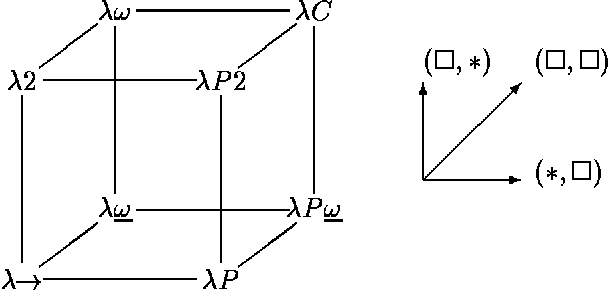
\includegraphics[scale=0.5]{pic.png}}
\end{center}

Выбор правил означает следующее:
\begin{itemize}
    \item $(*,\ *)$ - позволяет записывать термы, которые зависят от термов
    \item $(\openbox,\ *)$ - позволяет записывать термы, которые зависят от типов
    \item $(*,\ \openbox)$ - позволяет записывать типы, которые зависят от термов
    \item $(\openbox,\ \openbox)$ - позволяет записывать типы, которые зависят от типов
\end{itemize}

На самом деле в данной формулировке под типом понимается не только привычный тип. Потому что для привычного типа верно $\tau : *$. Здесь же $\tau$ может типизироваться чем угодно, кроме $\openbox$. В частности $* \rightarrow *$, это значит, что 
    
Также на этом кубике можно расположить языки программирования, например:
\begin{itemize}
    \item Haskell будет располагаться на левой грани куба, недалеко от $\lambda w$
    \item Idris и Coq, очевидно, будет находиться в $\lambda C$
    \item C++ очень ограниченно приближается к $\lambda C$ (мысли вслух):
    \begin{enumerate}
        \item $(*,\ *)$ - без этого не может обойтись ни один язык программирования
        \item $(\openbox,\ *)$ - например, sizeof(type)
        \item $(*,\ \openbox)$ - например, std::array<int, 19> - тут есть ограничение на то, значение каких типов можно подставлять.
        \item $(\openbox,\ \openbox)$ - например, std::vector<int>, int*
    \end{enumerate}
\end{itemize}

\subsection{Свойства}

Для систем в $\lambda$-кубе верны следующие утверждения:
\begin{itemize}
    \item \textbf{Th. SN} \qquad \qquad \qquad \quad \quad \ Обобщенная типовая система сильно нормализуема
    \item \textbf{Th. Черча-Россера} \quad \begin{minipage}{0.6\textwidth}
\raggedright % obviates the need for explicit linebreaks
\begin{enumerate}
    \item Для любых трёх элементов $A$, $B$ и $C$, таких, 
    $A \twoheadrightarrow B$ и $A \twoheadrightarrow C$ верно,
    что существует $D$, что 
    $B \twoheadrightarrow D$ и $C \twoheadrightarrow D$
    \item Для любых двух элементов $A$, $B$, для которых верно $A =_\beta B$, 
    существует $C$, что $A \twoheadrightarrow C$ и $B \twoheadrightarrow C$
\end{enumerate}
\end{minipage}
    \item \textbf{Th. Subject reduction} \quad \begin{minipage}{0.6\textwidth}
\raggedright % obviates the need for explicit linebreaks
    $\Gamma \vdash A : T$ и $A \twoheadrightarrow B$, тогда $\Gamma \vdash B : T$ 
\end{minipage}
    \item \textbf{Th. Unicity of types} \quad \ \  \begin{minipage}{0.6\textwidth}
\raggedright % obviates the need for explicit linebreaks
    $\Gamma \vdash A : T$ и $\Gamma \vdash A : T'$ тогда $T =_\beta T'$ 
\end{minipage}
\end{itemize}


\vspace{5mm}   

Примеры:

\begin{itemize}
    \item $\lambda \omega$:
\begin{center}
    $\vdash (\lambda \alpha : * . \alpha \rightarrow \alpha) : (* \rightarrow *) : \openbox$

\vspace{5mm}

\begin{enumerate}[]
    \item \begin{center}
        $\vcenter{\infer{\vdash (* \rightarrow *) : \openbox}{\vdash * : \openbox \qquad \infer{a:* \vdash *.\openbox}{\vdash *.\openbox} }}$
    \end{center}
    \item \begin{center} $\vcenter{\infer{\vdash (\lambda \alpha : * . \alpha \rightarrow \alpha) : * \rightarrow *}{\vdash * : \openbox \qquad \infer{\alpha : * \vdash \alpha \rightarrow \alpha : x}{\alpha : * \vdash \alpha : * \qquad \alpha : *, x : \alpha \vdash \alpha : *} \qquad \infer{a:* \vdash *: \openbox}{\vdash * :\openbox} } }$
    \end{center}
\end{enumerate}
\end{center}

% \item $\lambda \rightarrow$

\end{itemize}

Notes:
\begin{itemize}
    \item $(\lambda x.x) : (A \rightarrow A)$ - implicit typing (Curry style)
    \item $I_A = \lambda x : A.x$ - explicit typing (Church style)
\end{itemize}

Рассмотрим еще примеры для улучшения понимания лямбда-куба и обобщенной типовой системы:

\begin{itemize}
	
	\item В системе F ($\lambda 2$) выводимо:
	
	\begin{enumerate}
		\item $\vdash (\lambda \alpha : * . \lambda a : \alpha . a) : (\Pi \alpha : * . (\alpha \rightarrow \alpha)) : *$
		
		\item $A : * \vdash (\lambda \alpha : * . \lambda a : \alpha . a) A : (A \rightarrow A)$
		
		\item $A : *, b : A \vdash (\lambda \alpha : * . \lambda a : \alpha . a) A b : A$
		
		Разумеется, здесь имеет место редукция: $(\lambda \alpha : * . \lambda a : \alpha . a) A b \rightarrow_\beta b$.
	
	\end{enumerate}
	
	\item В $\lambda \underline{w}$ выполняется
	
	\begin{enumerate}
		\item $\vdash (\lambda \alpha : *. \alpha \rightarrow \alpha) : * \rightarrow * : \openbox$
		
		\item $\beta : * \vdash (\lambda \alpha : *. \alpha \rightarrow \alpha) \beta : *$
		
		\item $\beta : *, x : \beta \vdash (\lambda y : \beta . x) : (\lambda \alpha : *. \alpha \rightarrow \alpha) \beta$
		
		\item $a : *, f : * \rightarrow * \vdash f(fa) : *$
		
		\item $a : * \vdash (\lambda f : * \rightarrow * . f (f a)) : (* \rightarrow *) \rightarrow * $
	\end{enumerate}
	
	\item В $\lambda P$ верно:
	
	\begin{enumerate}
	    \item $A : * \vdash (A \rightarrow *) : \openbox$
	    
	    \item Рассмотрим тип A как множество значений типизируемых таким образом и введем $P : A \rightarrow *$
	    Тогда $A : *, P : A \rightarrow * , a : A \vdash P a : *$
	    Можно рассматривать в таком контексте P как предикат на А. Если для $a$ он возвращает населенный тип, то будем считать это за true, иначе за false. Это теоретико-множественный смысл зависимых типов.
	    
	    Можно строить утверждения вида $(\Pi a : A. P a)$ - для любого $a$ верен предикат P.
	    
	\end{enumerate}
	
    \item В $\lambda w$ можно задать конъюнкцию, как мы делали еще в системе F. $a \& b = \Pi \gamma : * . (a \rightarrow b \rightarrow \gamma) \rightarrow \gamma$
    
    Тогда $AND = \lambda a : *. \lambda b : *. a \& b$
    $K = \lambda a : *. \lambda b : *. \lambda x : a . \lambda y : b. x$
    
    $\vdash AND : * \rightarrow * \rightarrow *$
    
    $\vdash K : (\Pi a : *. \Pi b : *. a \rightarrow b \rightarrow a)$
    
    Тогда получается доказательство того, что из конъюнкции следует первый аргумент!
    
    $a : *, b : * \vdash (\lambda x : AND \: a b. x a (K a b)) : (AND \: a b \rightarrow a) : *$

\end{itemize}



\end{document}
